\documentclass[11pt, a4paper]{article}

\usepackage{geometry}
\geometry{
    textwidth=18cm, textheight=23.4cm,marginratio={1:1,5:7}      % actual formatting
    % left=1cm, right=5cm, vmargin={2.5cm,3cm}, marginparwidth=5cm   % todo-note friendly formatting (https://tex.stackexchange.com/a/156328)
}

% Load packages
\usepackage{booktabs}  % Nicer tables
\usepackage{rotating}  % For rotated table
\usepackage[table,xcdraw]{xcolor}  % Coloring
\usepackage{lineno}    % Line numbers
\usepackage[utf8]{inputenc}
\usepackage[english]{babel}
\usepackage[babel]{csquotes}
\usepackage{amsmath}
\usepackage{textcomp}
\usepackage{gensymb}   % for \degree
\usepackage{graphicx}
\usepackage{authblk}   % Multiple authors with affiliations
\usepackage{sidecap}   % for captions next to figures
\sidecaptionvpos{figure}{c}

% Color links
\usepackage{hyperref}
\hypersetup{
    colorlinks,
    linkcolor={red!50!black},                           % Color of within-text links (e.g., to a Figure)
    citecolor={blue!50!black},                          % Color of citation links (within text, to Bibliography)
    urlcolor={blue!50!black}                            % Color of URLs
}

% Set figure caption widths and fontsize
\usepackage{caption}
\captionsetup{
    width=0.85\textwidth,
    font=footnotesize,
    labelfont=bf,
    labelsep=period,
    justification=justified,
    singlelinecheck=false}

% Reference management
\usepackage[style=apa,doi=false,url=false,eprint=false]{biblatex}
\addbibresource{references.bib}

% \linenumbers  % uncomment to add line numbers

% Title page
\title{Gaze-dependent evidence accumulation predicts multi-alternative risky choice behaviour}

\author[1,2,*]{\small Felix Molter}
\author[3]{\small Armin W. Thomas}
\author[4,5]{\small Scott A. Huettel}
\author[2]{\small Hauke R. Heekeren}
\author[1,2]{\small Peter N. C. Mohr}
\affil[1]{\footnotesize School of Business \& Economics, Freie Universität Berlin, Berlin, Germany}
\affil[2]{\footnotesize Center for Cognitive Neuroscience, Freie Universität Berlin, Berlin, Germany}
\affil[3]{\footnotesize Center for Lifespan Psychology, Max Planck Institute for Human Development, Berlin, Germany}
\affil[4]{\footnotesize Center for Cognitive Neuroscience, Duke University, Durham, NC, USA}
\affil[5]{\footnotesize Department for Psychology and Neuroscience, Duke University, Durham, NC, USA}
\affil[*]{\footnotesize E-mail: \href{mailto:felixmolter@gmail.com}{felixmolter@gmail.com}}

\date{\today}

% Main document
\begin{document}

\maketitle

% Abstract
% ========
\abstract{Choices are influenced by gaze allocation during deliberation, so that fixating an alternative longer leads to increased probability of choosing it. Gaze-dependent evidence accumulation provides a parsimonious account of choices, response times and gaze-behaviour in many simple decision scenarios. Here, we test whether this framework can also predict more complex context-dependent patterns of choice in a three-alternative risky choice task, where choices and eye movements were subject to attraction and compromise effects. Choices were best described by a gaze-dependent evidence accumulation model, where subjective values of alternatives are discounted while not fixated. Finally, we performed a systematic search over a large model space, allowing us to evaluate the relative contribution of different forms of gaze-dependence and additional mechanisms previously not considered by gaze-dependent accumulation models. Gaze-dependence remained the most important mechanism, but participants with strong attraction effects employed an additional similarity-dependent inhibition mechanism found in other models of multi-alternative multi-attribute choice.}

% Main text
% =========

% Introduction
% ------------
\section*{Introduction}

% Gaze in binary risky choice
Imagine you inherited money from a distant relative and you need to decide how to invest it. You reach out to your trusted investment advisor who swiftly sends you a brochure with different investment alternatives. After reading the brochure, you look at the overview table provided on the final page and deliberate between two alternatives that particularly interest you, visually inspecting them, one at a time, comparing expected returns, associated risks, fees, and other attributes. Previous work has established that the role of visual attention in decision making under risk exceeds mere information sampling \parencite{glickman2019FormationPreferenceRisky,gluth2018ValuebasedAttentionalCapture,smith2018AttentionChoiceDomains}. Instead, as in other forms of preferential and perceptual decision making, visual fixations have a constructive role in the decision process, so that alternatives that are looked at for a longer time are generally more likely to be chosen \parencite{armel2008BiasingSimpleChoices,cavanagh2014EyeTrackingPupillometry,krajbich2010VisualFixationsComputation,parnamets2015BiasingMoralDecisions,shimojo2003GazeBiasBoth,sui2020TimingGazecontingentDecision,tavares2017AttentionalDriftDiffusion}.

This association between gaze and choice has been formalized in gaze-dependent evidence accumulation models \parencite[e.g.,][]{cavanagh2014EyeTrackingPupillometry,glickman2019FormationPreferenceRisky,gluth2018ValuebasedAttentionalCapture,krajbich2010VisualFixationsComputation,krajbich2011MultialternativeDriftdiffusionModel,molter2019GLAMboxPythonToolbox,thomas2019GazeBiasDifferences,tavares2017AttentionalDriftDiffusion}. The attentional Drift Diffusion Model \parencite[aDDM;][]{krajbich2010VisualFixationsComputation}, Gaze-weighted Linear Accumulator Model \parencite{molter2019GLAMboxPythonToolbox,thomas2019GazeBiasDifferences}, and others that apply explicitly to risky choice \parencite{glickman2019FormationPreferenceRisky} assume that decision makers accumulate evidence in favour of each alternative until evidence for one alternative reaches a threshold and a decision is made. Crucially, accumulation rates are assumed to depend on gaze allocation, so that evidence for an alternative is discounted while it is not fixated. Prior work has tested these assumptions in simple decisions under risk, involving two risky gambles with two equally probable outcomes \parencite{smith2018AttentionChoiceDomains} or two risky gambles described by outcome and probability \parencite{glickman2019FormationPreferenceRisky}. Like the example of choosing an investment plan, however, many real-life decisions are more complex than simple binary choice. For example, investment decisions can involve more than two alternatives that vary on multiple attributes (such as expected return, associated risk, and fees), including both sets of options with similarly low expected returns (e.g., government bonds, fixed deposits) and sets of other riskier options promising larger gains at higher risk (e.g., stocks or derivatives).

Crucially, choices in these multi-alternative, multi-attribute settings pose a challenge to many traditional models of risky choice, including Expected Utility Theory \parencite[EU][]{vonneumann1947TheoryGamesEconomic} and Prospect Theory \parencite{kahneman1979ProspectTheoryAnalysis,tversky1992AdvancesProspectTheory}, which obey basic axioms of rational choice like independence of irrelevant alternatives \parencite[IIA;][]{luce1959IndividualChoiceBehavior}. Briefly, IIA asserts that the preference between two alternatives should not depend on other alternatives. At least three context effects – the attraction \parencite{huber1982AddingAsymmetricallyDominated}, compromise \parencite{simonson1989ChoiceBasedReasons}, and similarity \parencite{tversky1972EliminationAspectsTheory} effects – show that IIA is frequently violated: The attraction effect describes an increase in preference for an alternative following the addition of a similar, but slightly inferior alternative. The compromise effect describes an increase in preference for an alternative after a third alternative was added that makes it appear as intermediate. The similarity effect predicts that adding a third option that is similar to one of the original options, and equally appealing, will increase relative preference for the other, dissimilar alternative. While these effects are predominantly investigated using consumer goods, some studies also found them to affect choices between risky gambles \parencite{huber1982AddingAsymmetricallyDominated,mohr2017AttractionEffectRisky,soltani2012RangeNormalizationModelContextDependent,tversky1972EliminationAspectsTheory,wedell1991DistinguishingModelsContextually}.

Generally, models that assume that each alternative can independently be assigned a single scale value denoting its utility \parencite[fixed utility or simple scalability models;][]{rieskamp2006ExtendingBoundsRationality} cannot account for the observed violations. In contrast, models that can predict the effects often assume that preferences are constructed by means of comparisons between alternatives on different attribute dimensions \parencite{roe2001MultialternativeDecisionField,trueblood2014MultiattributeLinearBallistic,tversky1972EliminationAspectsTheory,usher2004LossAversionInhibition,tversky1993ContextDependentPreferences}, and employ additional psychological or neurobiologically-inspired mechanisms, such as loss-aversion or inhibition between alternatives.

While current gaze-dependent accumulation models of risky choice assume that each alternative can be assigned a singular underlying scale value (e.g., expected utilities for each alternative), choices are also assumed to be constructed in an accumulation process that remains malleable due to its dependence on gaze. Therefore, gaze-dependent accumulation models potentially could account for violations of IIA or regularity if the distribution of gaze itself changed depending on the decision context (e.g., shift towards dominant alternatives in the attraction effect, compromise alternatives in the attraction effect, or dissimilar alternatives in the similarity effect). Initial evidence for such an attention-shift in the attraction effect comes from a study of intertemporal choice \parencite{marini2020AttractionComesMany}. Furthermore, recent work has suggested gaze-dependent evidence accumulation as a model of multi-alternative, multi-attribute choice in the absence of context effects \parencite{cohen2017MultiattributeMultialternativeModels,gluth2018ValuebasedAttentionalCapture}.

Here, we test to what extent gaze-dependent accumulation can explain risky choices in the presence of context effects. We replicate the attraction and compromise effects in a task where participants made repeated choices in a multi-alternative, multi-attribute setting involving risky gambles. We compare a model of gaze-dependent accumulation adapted from previous work on binary risky choice \parencite{glickman2019FormationPreferenceRisky} with an established model of context-dependent multi-alternative, multi-attribute choice without gaze-dependence and with other traditional models of risky choice. Notably, the gaze-dependent accumulation model did not include any dedicated mechanisms to produce context effects. Our task induced a set of context effects across the group, with substantial variability between individuals, providing a complex testing scenario to compare gaze-dependent accumulation models with competing theoretical accounts. We found the gaze-dependent model to give the overall best account of the choice data, while underestimating strong attraction effects of some individuals. A systematic search over a large model space combining features across model classes confirmed that all participants’ behaviour was best described by a gaze-dependent accumulation process, but that individual differences in attraction effect strengths are predicted best by variants integrating mechanisms from other models.

% Results
% -------
\section*{Results}

% Choice task
\subsection*{Choice task}

% Figure 1: Choice task and attribute space
\begin{SCfigure}[0.8]
\caption{\textbf{Choice task and attribute space of stimuli.} \textbf{(a)} Choice task. Trials started with a central fixation cross for 1.5 s. Next, three gambles were presented. Participants made a choice by button press, without time limit. Eye movements were recorded during the choice phase. Finally, brief feedback on the choice (but not on the gamble outcome) was displayed. \textbf{(b)} Attribute space. Each gamble is described by two attributes: Probability $p$ and outcome $m$. The core options $A$ and $B$ were presented in every trial, along with one of four decoy alternatives: Compromise decoys ($C_A$ or $C_B$) and asymmetrically dominated decoys ($D_A$ or $D_B$) are expected to elicit compromise and attraction effects, respectively. Dashed lines indicate possible stimulus placements. \textbf{(c)} Exact positions for $C_B$, $A$ and $C_A$ were calibrated for pairwise indifference in separate binary choice estimation blocks for each individual. Differences in outcome between neighbouring alternatives was not less than 2 EUR. Dominated decoys $D_A$ and $D_B$ were always 2\% and 1 EUR worse than $A$ and $B$ respectively.}
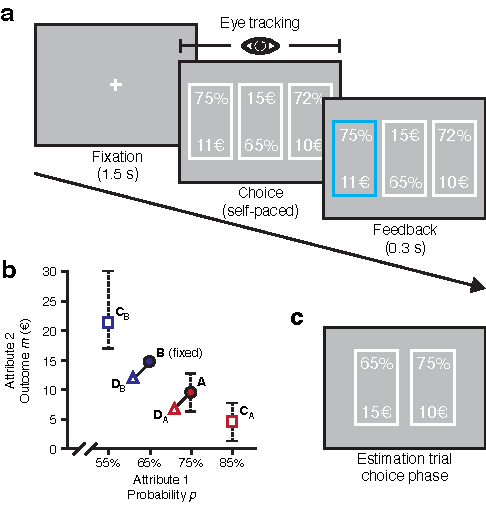
\includegraphics[scale=1]{../figures/1-task_stimuli.pdf}
\hspace{0.5cm}
\label{fig:task}
\end{SCfigure}

In our experiment, 40 participants made repeated decisions between three all-or-nothing gambles, each described by a probability $p$ to win an outcome $m$ and nothing otherwise (Figure \ref{fig:task}a). We recorded participants' eye movements during the task with an eye tracker (see \nameref{sec:methods} for details). Participants were instructed that after completing the task, their chosen gamble from one randomly determined trial would be played out for an additional bonus payment. In contrast to hypothetical choices between consumer goods described on attribute dimensions like quality and price, risky gamble stimuli offer a high amount of control over their attributes and a straightforward way to incentivise choices. The gamble stimuli were designed to elicit attraction and compromise effects and were individually tailored to account for each participant's risk preferences (Figure \ref{fig:task}b). Participants performed three pairs of indifference-estimation and experimental blocks, for a total of 225 experimental trials (see \nameref{sec:methods} for additional details on the experimental procedure and gamble stimuli). In indifference-estimation blocks, participants made repeated choices between pairs of gambles with different probabilities (Figure \ref{fig:task}c). Gamble outcomes $m$ were adjusted according to participants' choices so that four approximately equally preferred gambles $C_B$, $B$, $A$, and $C_A$ were constructed with winning probabilities $p$ = 55\%, 65\%, 75\%, and 85\%. Additionally, two asymmetrically dominated decoys $D_A$ and $D_B$ were defined to be 2\% and 1 EUR worse than gambles $A$ and $B$, respectively. Following this indifference estimation, participants performed an experimental block of 75 ternary choice trials, 32 of which were compromise trials balanced with respect to the target option (i.e., 16 choice sets \{$A$, $B$, $C_A$\}, 16 choice sets \{$A$, $B$, $C_B$\}), 32 attraction trials (16 choice sets \{$A$, $B$ ,$D_A$\}, 16 choice sets \{$A$, $B$, $D_B$\}) and 11 distractor trials showing randomly created options with expected value of 10 EUR and low (5–33\%), medium (34–64\%) and high (65–95\%) probability $p$. Uniform noise was added to all outcomes $m$ ($\pm$0 EUR, +1 EUR) and probabilities $p$ (–3\%, $\pm$0\%, +3\%) in each trial. Asymmetrically dominated decoys $D_A$ and $D_B$ received the same noise as the target option to preserve the dominance relation.

\subsection*{Context effects}

% Table 1: Choice frequencies
\begin{table}[bt!]
\begin{centering}
\begin{tabular}{@{}llll@{}}
\toprule
\textbf{Trial type} & \textbf{Target} & \textbf{Competitor} & \textbf{Decoy} \\ \midrule
$D_A$               & 0.60            & 0.39                & 0.01           \\
$D_B$               & 0.53            & 0.45                & 0.02           \\
$C_A$               & 0.46            & 0.37                & 0.16           \\
$C_B$               & 0.32            & 0.31                & 0.37           \\ \bottomrule
\end{tabular}
\caption{\textbf{Relative choice frequencies across participants in the four trial types.} Across the group, target options were chosen more frequently than competitors in both types of attraction ($D_A$ and $D_B$) and compromise trials ($C_A$, $C_B$). Dominated decoys were almost never chosen. In compromise trials including the high-outcome decoy $C_B$ , the decoy was chosen more frequently than core options.}
\label{tab:choicefreqs}
\end{centering}
\end{table}

We first analysed participants' choice behaviour to test whether their choices could be influenced by the set of available alternatives (see Table \ref{tab:choicefreqs} and Figure \ref{fig:cfx}). Participants rarely chose the dominated decoys in attraction trials (mean $\pm$ s.d. = 0.02 $\pm$ 0.02 of attraction trials), indicating that participants understood the dominance relationships among the stimuli. In compromise trials, participants chose (non-dominated) decoy alternatives more frequently (mean $\pm$ s.d. = 0.27 $\pm$ 0.16). In particular, the decoy with the highest possible outcome $C_B$ ($p \approx$ 55\%, $m \approx$ 18 EUR) was chosen most frequently when it was available. Note that decoy choices in compromise trials are expected, as extreme decoys were specifically calibrated to be approximately equally preferred to the core options. 

We tested the presence of the attraction and compromise effects by first computing the relative choice share of the target alternative \parencite[RST;][]{berkowitsch2014RigorouslyTestingMultialternative} for each individual, and separately for attraction and compromise trials. The RST is computed as

\begin{equation}
    RST = \frac{N_{\text{target}}}{N_{\text{target}} + N_{\text{competitor}}}
\end{equation}

where $N$ is the number of times an alternative was chosen. Given the balanced design, where each core alternative acts as a target and competitor equally often, the RST should be close to 0.5 if no context effects are present. If, however, the RST is different from 0.5, a systematic context effect is indicated. We tested whether the mean RST significantly differed from 0.5 across participants by computing its 95\% highest posterior density interval (HDI$_{95}$) using Bayesian estimation \parencite[BEST;][]{kruschke2013BayesianEstimationSupersedes,kruschke2014DoingBayesianData}. 

We find evidence for the attraction effect: The mean RST in attraction trials differed meaningfully from 0.5 (mean RST = 0.56, HDI$_{95}$ = [0.51, 0.60], mean $d$ = 0.49, HDI$_{95}$ = [0.10, 0.80]). 25 of 40 (62.5\%) participants had an RST above 0.5 in attraction trials. Notably, similar to previous work \parencite[e.g.,][]{trueblood2012MultialternativeContextEffects} a subgroup of participants (9 of 40, 22.5\%) showed particularly strong attraction effects with individual RSTs above 0.7. We could not, however, find evidence that these individuals used the dominance relationship as a simplifying choice rule (see \nameref{sec:supplement}). To allow comparisons with other studies that quantified context effects as the difference between choice shares between targets and competitors, we also report these differences: In attraction trials, the average difference was 0.12 (HDI$_{95}$ = [0.01, 0.20], mean $d$ = 0.48, HDI$_{95}$ = [0.11, 0.85], Figure \ref{fig:cfx}b). 

We only found weak evidence for the compromise effect using the gamble stimuli: The mean RST in compromise trials was 0.53, but its estimated HDI$_{95}$ did not exclude 0.5 (HDI$_{95}$ = [0.49, 0.57], 91.1\% of posterior mass above 0.5, mean $d$ = 0.23, HDI$_{95}$ = [-0.11, 0.59]). 26 of 40 (65\%) participants showed an RST above 0.5 in compromise trials. The mean difference between choice shares for targets and competitors was 0.05 (HDI$_{95}$ = [-0.01, 0.11], mean $d$ = 0.29, HDI$_{95}$ = [-0.04, 0.62], 95.8 \% of posterior mass above 0; Figure \ref{fig:cfx}e). These results are similar to the marginal effects obtained using perceptual stimuli in previous work \parencite{trueblood2015FragileNatureContextual,trueblood2013NotJustConsumers}. 

Similar to other work \parencite{berkowitsch2014RigorouslyTestingMultialternative,trueblood2014MultiattributeLinearBallistic}, we found a positive correlation between the effects across participants, even though it was weaker in our task ($r$ = 0.24, HDI$_{95}$ = [-0.05, 0.51], 94.5\% of posterior mass above 0). 

Taken together, we successfully induced context effects within our participant sample, with non-trivial variability in the strength of those effects across individuals. These data provide a complex testing scenario to investigate gaze-bias effects in multi-alternative multi-attribute choice and to compare gaze-dependent accumulation models with competing theories.

% Figure 2: Context effects in choices and relative dwell times
\begin{figure}[bt!]
\begin{centering}
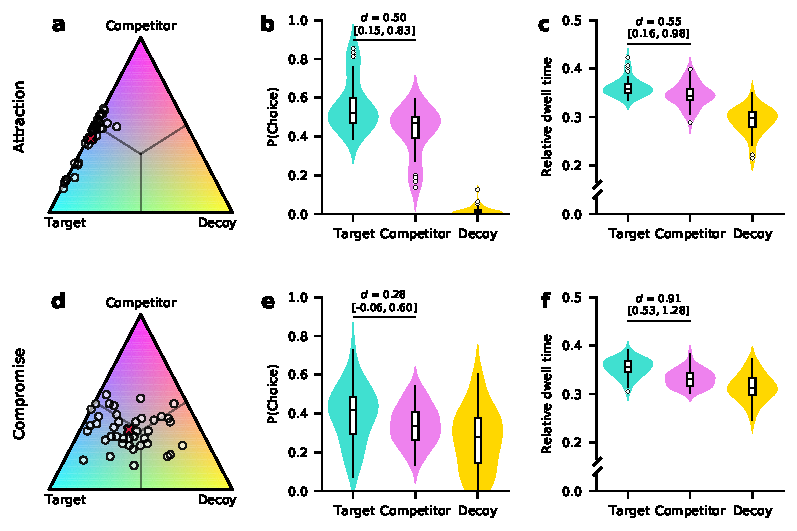
\includegraphics[scale=1]{../figures/2-context-effects.pdf}
\caption{\textbf{Context effects are present in choices and relative dwell time.} Participants choices were influenced by asymmetrically dominated decoys and, to a lesser extent, by extreme compromise-making decoys. \textbf{(a, d)} Ternary plots of individual relative choice frequencies for target (lower left, teal), competitor (top, pink), and decoy (lower right, yellow) alternatives in attraction \textbf{(a)} and compromise \textbf{(d)} trials. Each dot represents one participant. The position on the simplex indicates relative choice frequencies for alternatives. Straight lines from the centre indicate equal frequencies for two alternatives. The red "x" indicates the group average. \textbf{(b, e)} Relative choice frequencies in attraction \textbf{(b)} and compromise \textbf{(e)} trials. In attraction trials, some participants strongly favoured the target alternative and almost no decoy choices were made. While target alternatives are still chosen more frequently than competitors in compromise trials, the effect is less pronounced, and extreme decoys are still chosen frequently. \textbf{(c, f)} Relative dwell time towards alternatives. In both, attraction \textbf{(c)} and compromise \textbf{(f)} trials, target alternatives received greater relative dwell times than competitors. $d$ denotes Cohen's $d$ from paired BEST analysis with HDI$_{95}$ given in brackets. Violin plots show kernel density estimates of distributions of individual values. Box plots mark lower and upper quartiles and median. Whiskers extend from first and last datum within 1.5 times the interquartile range from lower and upper quartiles, respectively. Values outside this range are indicated by open circles.}
\label{fig:cfx}
\end{centering}
\end{figure}

\subsection*{Context effects are present in relative dwell times}

Next, we tested whether participants' eye movements were affected by the set of available alternatives, similar to their choices. We therefore computed each alternative's relative dwell time in a trial by summing the duration of all fixations durations towards it, and normalizing to the sum of all fixations in the trial. Both patterns of context effects of choice behaviour were present in the relative dwell data: Target options received greater relative dwell time than competitors in attraction (mean difference = 0.015, HDI$_{95}$ = [0.005, 0.4], mean $d$ = 0.55, HDI$_{95}$  = [0.16, 0.98], Figure \ref{fig:cfx}c) and compromise trials (mean difference = 0.022, HDI$_{95}$  = [0.014, 0.03], mean $d$ = 0.91, HDI$_{95}$  = [0.53, 1.28], Figure \ref{fig:cfx}f). Targets and competitors also received greater relative dwell time than decoys in both trial types.

To better understand participants' eye movements over the course of the trial, we performed additional exploratory analyses of gaze location and transitions. We found an increasing association between gaze and choice over the trial, and longer gaze towards targets, even accounting for choice. Information search occurred both within and between alternatives, with slightly more transitions within alternatives. We refer to the \nameref{sec:supplement} for additional details on these analyses.

\subsection*{Behavioural modeling and model comparison}

% Figure 3: Model comparison results, predicted gaze-choice association RST prediction of winning model
\begin{figure}[bt!]
\begin{centering}
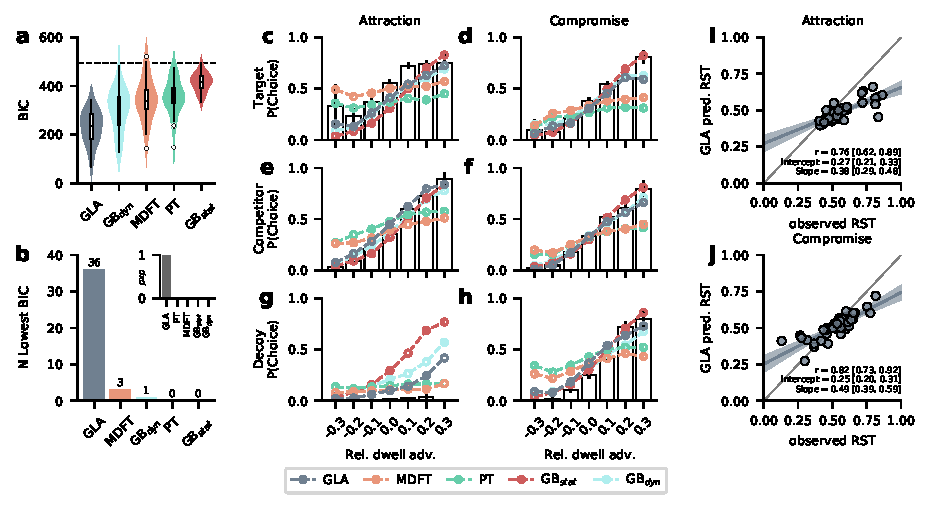
\includegraphics[scale=1]{../figures/3-model-comparison.pdf}
\caption{\textbf{Model comparison and predictions.} \textbf{(a)} The gaze-dependent leaky accumulator (GLA) provided the best fit (lowest mean BIC) across participants, followed by the dynamic gaze baseline model, MDFT, EU, and the static gaze baseline model. The dashed line indicates the BIC of the random choice baseline model. Violin plots show kernel density estimates of distributions of individual values. Box plots mark lower and upper quartiles and median. Whiskers extend from first and last datum within 1.5 times the interquartile range from lower and upper quartiles, respectively. Values outside this range are indicated by open circles. \textbf{(b)} The GLA fitted most (36 of 40, 90\%) participants best, with a protected exceedance probability of 1 (inset). \textbf{(c-h)} Observed and model-predicted probability of choosing the target \textbf{(c, d)}, competitor \textbf{(e, f)}, or decoy \textbf{(g, h)} alternatives in attraction \textbf{(c, e, g)} and compromise trials \textbf{(d, f, h)} as a function of relative dwell time advantage. Relative dwell time advantage was computed as relative dwell time towards an alternative minus the mean relative dwell time to all other alternatives. White bars and error bars show mean $\pm$ s.e. observed data from even-numbered trials. Model predictions (coloured lines) are based on 50 simulations of each odd-numbered trial. \textbf{(i, j)} Observed and predicted RST of the best-fitting GLA for attraction \textbf{(i)} and compromise \textbf{(j)} trials. Each circle represents one participant. The winning model’s predicted context effect sizes correlated significantly with the observed ones. Strong context effects, however, were underestimated, as indicated by the reduced slopes.}
\label{fig:modelcomparison}
\end{centering}
\end{figure}

Given that participants’ choices and eye movements exhibited modulation by the context of available options, we next tested whether their behaviour could be described using a gaze-dependent accumulation model, and how such a model performs in comparison to extant theories of multi-alternative multi-attribute choice. To this end, we adapted a recently developed, gaze-dependent leaky accumulator model of two-alternative risky choice \parencite{glickman2019FormationPreferenceRisky} to the three-alternative scenario. We refer to this model as the Gaze-dependent Leaky Accumulator (GLA). It assumes that subjective utilities for each alternative $i$ are constructed as in Cumulative Prospect Theory \parencite{tversky1992AdvancesProspectTheory} by first applying a probability weighting function, that transforms objective probabilities $p$ into subjective decision weights. Outcomes $m$ are transformed into utilities using a power function. Next, this model assumes that for each alternative $i$ subjective utilities $x_i^{GLA}$ are accumulated with leakage over the time course of each trial and that utilities are discounted while they are not fixated. At each fixation $n$, accumulators evolve according to

\begin{equation}
    \label{eq:gla:accumulator}
    X_i^{GLA}(n) = \begin{cases}
             (1 - \lambda) \cdot X_i^{GLA}(n - 1) + 1 \cdot x_i^{GLA} &\text{if $i$ fixated}\\
             (1 - \lambda) \cdot X_i^{GLA}(n - 1) + \theta \cdot x_i^{GLA} &\text{otherwise}
             \end{cases}
\end{equation}

where all $X_i(0)=0$. Similar to the aDDM, the $\theta$ parameter ($0 \le \theta \le 1$) controls discounting of unattended alternative utilities. The $\lambda$ parameter ($0 \le \lambda \le 1$) controls the strength of the accumulation leak. We computed choice probabilities from this model by applying the soft-max choice rule (Equation \ref{eq:softmax}) over the final accumulator values $X_i^{GLA}$.

Additionally, we fitted an implementation of Multialternative Decision Field Theory \parencite[MDFT;][]{roe2001MultialternativeDecisionField}, representing the class of dynamic multi-attribute, multi-alternative choice theories that have been designed to explain context effects. In contrast to GLA, MDFT assumes that preferences evolve dynamically over time by accumulation of attribute-wise comparisons between alternatives, and alternatives inhibit each other depending on their distance (or similarity). MDFT does not assume any influence of gaze on the decision process. We also included three baseline models in our comparison. First was a standard Expected Utility model \parencite[EU;][]{vonneumann1947TheoryGamesEconomic} that did not consider gaze data. Second, a static gaze baseline model GB$_{\text{stat}}$ predicted choices only from trial-aggregated gaze towards each alternative, ignoring outcome values and outcome probabilities. Third, we constructed a dynamic gaze baseline model GB$_{\text{dyn}}$ that, like GLA, assumed leaky evidence accumulation over fixations, but ignored attribute values, using only the sequence of fixations in each trial to predict choices. See \nameref{sec:methods} for details on these models' implementation and parameter estimation.

All models were fit individually to the choice data of each participant. We compared the models using the Bayesian Information Criterion \parencite[BIC;][]{schwarz1978EstimatingDimensionModel}, which penalizes more complex models and therefore accounts for differences in complexity between models.

Across the group, all models performed better than the random baseline model (Figure \ref{fig:modelcomparison}a). The GLA had the lowest BIC (mean $\pm$ s.d. = 230.63 $\pm$ 66.80), followed by the dynamic gaze baseline model GB$_{\text{dyn}}$ (mean $\pm$ s.d. = 302.46 $\pm$ 86.15), MDFT (mean $\pm$ s.d. = 345.77 $\pm$ 82.44), EU (mean $\pm$ s.d. = 360.57 $\pm$ 72.56) and the static gaze baseline GB$_{\text{stat}}$ (mean $\pm$ s.d. = 414.81 $\pm$ 36.81). Simulating choices from the models using maximum-likelihood estimates, the proportion of correctly predicted choices was 74.2\% for GLA, 62.8\% for GB$_{\text{dyn}}$, 57.9\% for MDFT, 53.8\% for EU and 45.7\% for GB$_{\text{stat}}$ (see Supplementary Figure \ref{fig:model-pred-probs} for distributions of model-predicted choice probabilities). Note, that target and competitor options (and decoys in compromise trials) were designed to be closely matched in value, resulting in trials with high choice difficulty, limiting overall model performance. On the individual level, based on lowest BIC scores, the majority (36 of 40, 90\%) of participants were best described by GLA. Three participants (7.5\%) were best described by MDFT, and one by the dynamic gaze-baseline model (Figure \ref{fig:modelcomparison}b). Protected exceedance probabilities \parencite{rigoux2014BayesianModelSelection}, which measure the likelihood that model is more frequent than all others, unambiguously identified GLA as the most likely model (pXP$_{\text{GLA}}$ = 1, Figure \ref{fig:modelcomparison}b inset).

The estimates for GLA’s gaze-discount parameter $\theta$, which describes the degree to which alternative’s values are attenuated while not fixated, indicate that participants exhibited a moderate gaze-discount on average: $\theta$ estimates ranged from 0.13 (strong gaze-discount) to 0.95 (almost no gaze-discount), with mean $\pm$ s.d. = 0.69 $\pm$ 0.18. Estimates for the leak parameter ranged from 0.08 (almost no leak) to 0.65 (moderately strong leak), with mean $\pm$ s.d. = 0.29 $\pm$ 0.2. Individual parameter estimates of all GLA parameters are plotted in Supplemental Figure \ref{fig:gla-estimates} and summarised in Supplemental Table \ref{tab:gla-estimates}.

Given that MDFT outperforms utility-based models when choices are influenced by context \parencite{berkowitsch2014RigorouslyTestingMultialternative}, we tested whether model fit of MDFT (relative to GLA) was higher for participants with higher RST. In other words: Does MDFT perform better for stronger context effects? Overall, 7 out of 9 participants with an RST above 0.7 in attraction trials were clearly best described by GLA. While we found that the relative superiority of GLA over MDFT decreased with strong attraction effects, this was not the case for compromise trials (Supplemental Figure \ref{fig:dbic-rst}), suggesting that some features of MDFT might help capture strong attraction effects.

As an additional indicator of model fit, we tested whether the models could quantitatively reproduce the observed positive association of gaze and choice (Supplemental Figures \ref{fig:dwell-data-timebinned}d, j, \ref{fig:dwell-regression-weights}). Specifically, following previous work \parencite{krajbich2010VisualFixationsComputation,krajbich2011MultialternativeDriftdiffusionModel}, we inspected the model-predicted probability of choosing an alternative as a function of its relative dwell time advantage: the difference in relative dwell time towards an alternative minus the mean relative dwell time to other alternatives. The probability of choosing an alternative generally increased with its relative dwell time advantage (Figure \ref{fig:modelcomparison}c-h), except for dominated decoys in attraction trials, which were not chosen even if looked at longer than other alternatives (Figure \ref{fig:modelcomparison}g).

All gaze-dependent models were able to capture this positive association. Note, however, that they also predicted choices of dominated decoys in attraction trials, if decoys had a large dwell time advantage (Figure 3g). In this case, GLA performed better than GB$_{\text{dyn}}$ and GB$_{\text{stat}}$, as it predicted fewer decoy choices. However, MDFT and EU generally could not capture the empirical association of gaze and choice; they predicted too many choices of alternatives with negative dwell time advantage, and too few choices of alternatives with positive dwell time advantage. 
Nor did they predict choices of dominated decoys, even if the decoy was looked at longer.

Finally, we investigated the ability of the best-performing model to predict individual differences in context effect strengths. Therefore, we predicted choices from the fitted GLA model and correlated the resulting RST with the observed data. Predicted RST correlated significantly with observed ones in attraction ($r$ = 0.63, HDI$_{95}$ = [0.43, 0.79], Figure \ref{fig:modelcomparison}i) and compromise ($r$ = 0.73, HDI$_{95}$ = [0.58, 0.86], Figure \ref{fig:modelcomparison}j) trials. However, the model underestimates large deviations from RST = 0.5, suggesting that its gaze-discount mechanism can capture the qualitative pattern of context effects but not their expression in participants with extreme RSTs. 

Inspection of predicted choice probabilities (Supplemental Figure \ref{fig:model-pred-probs}) shows that, on average, GLA predicted high probabilities for the empirically chosen alternative (indicating good overall fit), but comparable proportions of target and competitor choices (resulting in reduced RST). Other models, like MDFT, predicted larger differences between target and competitor choices for some participants, but assigned lower probability to empirically chosen alternatives (resulting in overall inferior fit).

% Switchboard Analysis
\subsection*{Systematic exploration of a large model space}

% Motivation
The model comparison identified the advantage of the gaze-dependent accumulation model over its competitors. To better understand the contribution of individual model mechanisms (such as accumulation leak, inhibition between alternatives, or the gaze-dependent discount) to model performance, we performed a search across a large, systematically designed model space, in a so-called "switchboard analysis" \parencite[see][]{turner2018CompetingTheoriesMultialternative}. Here, the idea is to isolate, group and exhaustively combine mechanistic assumptions of different models. Each group of mechanisms is considered a switch that can take different levels (e.g., an "inhibition" switch could take the levels "distance-dependent" as in MDFT, "constant" or "none"). Ultimately, this approach can be used to gauge the contribution of individual model mechanisms (opposed to evaluating whole models or model classes as in the more traditional model comparison presented above). In addition, it provides a systematic way to generate novel hybrid models, combining mechanisms from different \emph{a priori} defined models.

This analysis approach further allowed us to test different assumptions about the functional forms of the gaze bias mechanism \parencite[e.g., as discounting non-fixated alternatives’ values, controlling accumulation leak, among others; see][]{ashby2016FindingRightFit}. We therefore expanded the range of gaze-dependent mechanisms from the original set of models to include additional eye-movement related switches, like attribute- and alternative-wise gaze-discounts, gaze-dependent leakage and inhibition. This allowed us to test if gaze-bias implementations different from the ones usually used in gaze-dependent accumulation \parencite{fisher2017AttentionalDriftDiffusion,krajbich2010VisualFixationsComputation,krajbich2011MultialternativeDriftdiffusionModel,krajbich2012AttentionalDriftdiffusionModel,molter2019GLAMboxPythonToolbox,thomas2019GazeBiasDifferences,smith2018AttentionChoiceDomains,tavares2017AttentionalDriftDiffusion}.

Our switchboard comprised a total of 192 model variants, derived from six switches that were combined exhaustively: Attribute integration (additive vs. multiplicative), evidence comparison (independent accumulation for each alternative or comparative accumulation of evidence relative to other alternatives), alternative-wise and attribute-wise gaze-discount (included or not), accumulation leak (none, constant or gaze-dependent) and inhibition between alternatives (none, constant, gaze-dependent or distance-dependent). The models generally resembled the form of the \emph{a priori} defined GLA, but with substantial differences depending on the specific set of switch levels (Figure \ref{fig:switchboard}a; see \nameref{sec:methods} and Supplemental Table \ref{tab:switchboard-overview} for details on the framework and switch levels). As before, each model variant was fit to the individual data of each participant and model performance was evaluated based on the BIC score. Note that the GLA coincides with one of the 192 variants (variant A in Table \ref{tab:switchboard-best-ind}; multiplicative attribute integration, alternative-wise gaze-discount, constant leak, no inhibition, no comparison). Similarly, one variant (not in Table \ref{tab:switchboard-best-ind}) conceptually resembles MDFT in some, but not all aspects (additive attribute integration, comparative evidence accumulation, constant leak, distance-based inhibition, strong attribute-wise gaze-discount).

% Figure 4: Switchboard analysis overview
\begin{figure}[t!]
\begin{centering}
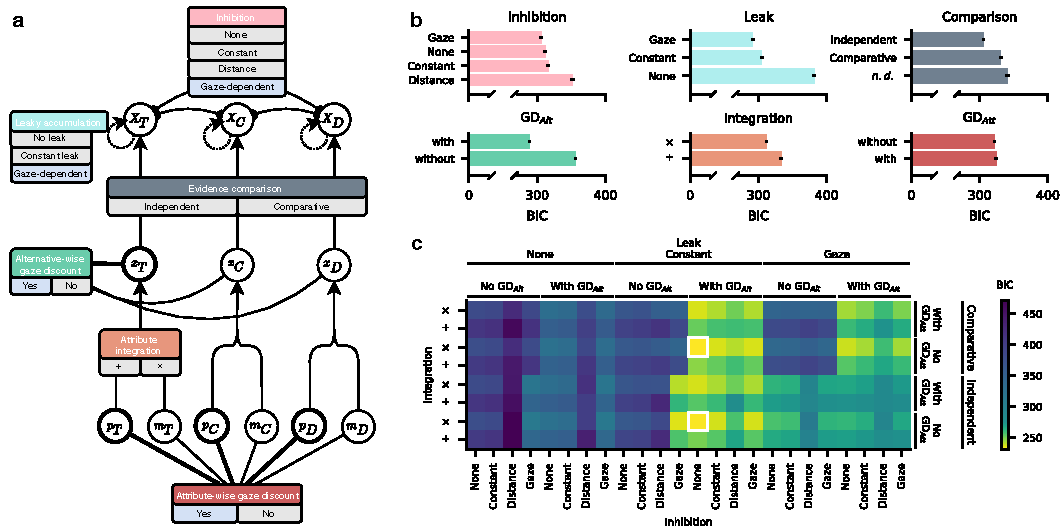
\includegraphics[scale=1]{../figures/4-switchboard.pdf}
\caption{\textbf{Switchboard analysis.} \textbf{(a)} Overview of general switchboard framework and individual switches from which individual variants are constructed by setting the switches to a set of levels. Gaze-dependent switch levels are shaded blue. Attributes can be discounted based on gaze (lower level) and are integrated into alternative values (middle level). Alternative values can be discounted based on gaze, compared, and integrated (upper level) with leak and inhibition. \textbf{(b)} Average model fit associated with each switch’s levels. Each bar shows the average BIC for all model variants that had the respective switch set to this level (e.g., first panel, top bar: average BIC of all variants with gaze-dependent inhibition). Gaze-dependent inhibition and leak, independent evidence accumulation, alternative-wise gaze-discount, multiplicative attribute integration, and no attribute-wise gaze-discount yielded lower BIC on average. \textbf{(c)} Overview of mean BIC for each of 192 model variants. More yellow colours indicate lower BIC and better model fit. The variant with the lowest BIC is identical to the GLA (alternative-wise, no attribute-wise gaze-discount, multiplicative attribute integration, constant leak, and no inhibition) and is outlined in white. Note that some variants were mathematically equivalent (see main text and Methods) including the variant with lowest BIC, which is therefore highlighted twice.}
\label{fig:switchboard}
\end{centering}
\end{figure}

\subsubsection*{Best model mechanisms}

On the level of model mechanisms, multiplicative attribute integration outperformed additive integration (mean BIC$_{\text{mul.}}$ = 312.25, mean BIC$_{\text{add.}}$ = 333.20; Figure 4b), inclusion of an alternative-wise gaze-discount (mean BIC$_{\text{GD alt.}}$ = 289.13, mean BIC$_{\text{no GD alt.}}$  = 356.32), but not attribute-wise gaze-discount yielded lower BIC scores (mean BIC$_{\text{GD att.}}$  = 324.11, mean BIC$_{\text{no GD att.}}$ = 321.33). Other gaze-dependent mechanisms also improved model fit: Variants with gaze-dependent leak yielded lower BIC scores than variants with constant or no leak (BIC$_{\text{gaze}}$  = 292.06, BIC$_{\text{constant}}$ = 304.84, BIC$_{\text{none}}$ = 381.49). Gaze-dependent inhibition performed better than constant, none or distance-dependent inhibition (BIC$_{\text{gaze}}$ = 305.64, BIC$_{\text{constant}}$ = 316.06, BIC$_{\text{none}}$ = 311.75, BIC$_{\text{distance}}$ = 351.57). In summary, all mechanisms that allowed a model to exploit the positive association between gaze and choice improved model fit on average.

Counting switch-values of individually best fitting variants, most participants were best described by model variants with multiplicative integration, with alternative-wise and no attribute-wise gaze-discount, with constant accumulation leak parameter and no inhibition (Supplemental Figure \ref{fig:switchboard-ind-switch-counts}).

\begin{table}[ht!]
\centering
\begin{tabular}{@{}cccccccc@{}}
\toprule
 & \textbf{$N$} & \textbf{GD$_{\text{Alt}}$} & \textbf{GD$_{\text{Att}}$} & \textbf{Leak} & \textbf{Inhibition} & \textbf{Integration} & \textbf{Comparison} \\ \midrule
A & 17 & \cellcolor[HTML]{DAE8FC}Yes & No & Constant & None & Multiplicative & \textit{n.d.} \\
B & 9 & \cellcolor[HTML]{DAE8FC}Yes & No & Constant & Distance & Multiplicative & Comparative \\
C & 4 & \cellcolor[HTML]{DAE8FC}Yes & No & Constant & None & Additive & \textit{n.d.} \\
D & 3 & No & No & \cellcolor[HTML]{DAE8FC}Gaze & None & Multiplicative & Independent \\
E & 2 & No & No & Constant & \cellcolor[HTML]{DAE8FC}Gaze & Multiplicative & Independent \\
F & 1 & \cellcolor[HTML]{DAE8FC}Yes & No & \cellcolor[HTML]{DAE8FC}Gaze & Distance & Multiplicative & Comparative \\
G & 1 & \cellcolor[HTML]{DAE8FC}Yes & No & \cellcolor[HTML]{DAE8FC}Gaze & Constant & Multiplicative & Comparative \\
H & 1 & \cellcolor[HTML]{DAE8FC}Yes & \cellcolor[HTML]{DAE8FC}Yes & Constant & Distance & Multiplicative & Independent \\
I & 1 & \cellcolor[HTML]{DAE8FC}Yes & No & Constant & \cellcolor[HTML]{DAE8FC}Gaze & Multiplicative & Comparative \\
J & 1 & \cellcolor[HTML]{DAE8FC}Yes & No & \cellcolor[HTML]{DAE8FC}Gaze & None & Multiplicative & Comparative \\ \bottomrule
\end{tabular}
\caption{\textbf{Overview of individually best fitting model variants.} $N$ indicates the number of participants best described by the variant described in the row. The top variant (A) coincided with the GLA model. Note that all individually best fitting models had some form of gaze-dependence (blue shaded cells, mostly alternative-wise gaze-discount). \emph{"n.d."} denotes variants where comparison mechanisms were not distinguishable by the analysis.}
\label{tab:switchboard-best-ind}
\end{table}

\subsubsection*{Best model variants}

The overall best-fitting model variant was the variant identical to the GLA (Figure \ref{fig:switchboard}c, Supplemental Table \ref{tab:switchboard-best-agg}): It included multiplicative attribute integration, an alternative-wise gaze-discount, and constant leak. Note that our analysis did not allow us to distinguish independent and comparative accumulation for this variant, because they yield equivalent results. All of the ten best performing models used multiplicative attribute integration, and most used an alternative-wise but no attribute-wise gaze-discount and constant leak (Supplemental Table \ref{tab:switchboard-best-agg}). Results were more ambiguous for the comparison and inhibition mechanisms.

Notably, one of the best ten variants employed a distance-dependent inhibition mechanism, and used other features resembling MDFT like constant leak, and accumulation of comparative values. Unlike MDFT, but like GLA, this variant used an alternative-wise gaze-discount, no attribute-wise mechanism of attention, and multiplicative integration of attributes. While not achieving the best overall fit, this hybrid variant performed significantly better than the original MDFT implementation (mean BIC$_{\text{MDFT}}$ = 345.77; Figure \ref{fig:modelcomparison}a).

The GLA variant also described 17 of 40 (42.5\%) participants best (Table \ref{tab:switchboard-best-ind}). Another similar variant with additive attribute integration described an additional four participants best. An additive relationship between attributes is typically assumed by models of multi-attribute multi-alternative choice \parencite[e.g.,][]{roe2001MultialternativeDecisionField,usher2004LossAversionInhibition}. Furthermore, additive integration of probability and outcome has recently been suggested as an alternative to multiplicative mechanisms and has been demonstrated to be equivalent for particular parameterizations and parameter values \parencite{rouault2019PrefrontalMechanismsCombining}. Five participants were best described by variants similar to the GLA, but using gaze-dependent leakage or inhibition instead of an alternative-wise gaze-discount. Note that gaze-dependent inhibition and leakage mechanisms can act similarly to an alternative-wise gaze-discount: All three mechanisms effectively reduce accumulated evidence of non-fixated alternatives. While the alternative-wise gaze bias mechanism applies a constant discount to the accumulation inputs, the gaze-dependent inhibition mechanism is proportional to the accumulated evidence of the currently fixated alternative, and applies to the already accumulated evidence of other options, not the inputs to the accumulation process. Gaze-dependent leakage similarly reduces already accumulated evidence, proportional to the momentary accumulator value.

Notably, nine participants (22.5\%) were best described by the previously described hybrid variant using a distance-dependent inhibition mechanism (Table \ref{tab:switchboard-best-ind}). Additional two participants were best described by other variants using distance-dependent inhibition in conjunction with an alternative-wise gaze-discount.

% Figure 5: Hybrid variant
\begin{SCfigure}[0.6][tb]
\caption{\textbf{Hybrid model variant details.} \textbf{(a, b)} Number of participants better described by the hybrid variant (pink) or the GLA (grey), dependent on strength of attraction \textbf{(a)} and compromise \textbf{(b)} effects. Participants with strong attraction effects were better described by the hybrid variant. \textbf{(c, d)} Individual observed and predicted RST in attraction \textbf{(c)} and compromise trials \textbf{(d)}. Compared to GLA (Figure \ref{fig:modelcomparison}i, j), the hybrid model better predicted strong attraction effects for some participants. Predictions of compromise effects are similar. \textbf{(e, f)} Observed and model-predicted probability of choosing the target alternative, depending on the target’s relative dwell time advantage. Like other gaze-dependent models (Figure \ref{fig:modelcomparison}), the hybrid variant generally captured the positive association between gaze and choice. In contrast to GLA, however, it predicted an overall higher probability of choosing the target in attraction trials \textbf{(e)}. Predictions in compromise trials \textbf{(f)} are similar to GLA. White bars and error bars indicate mean $\pm$ s.e. observed data from even-numbered trials. Model predictions are based on 50 simulations for each odd-numbered trial.}
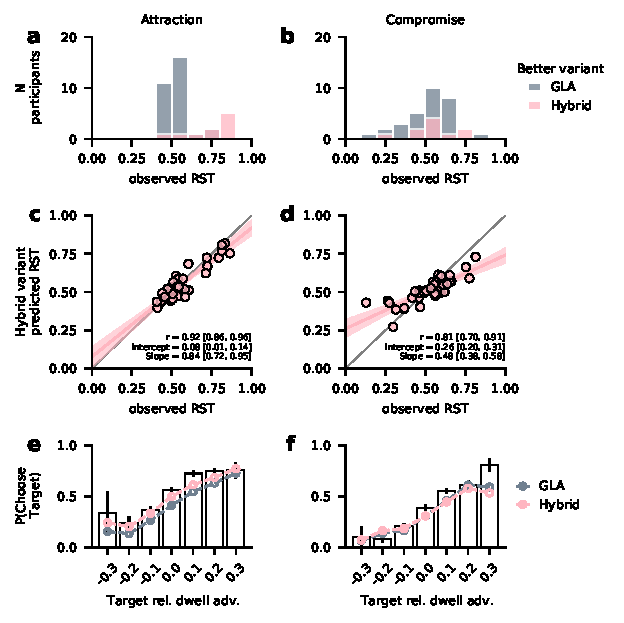
\includegraphics[scale=1]{../figures/5-hybrid-variant.pdf}
\label{fig:hybrid}
\end{SCfigure}

\subsubsection*{Hybrid variant}

Finally, we analysed the hybrid model variant in more detail (variant B in Table \ref{tab:switchboard-best-ind}), which described 9 participants best. This variant performed especially well for participants with large attraction effects (Figure \ref{fig:hybrid}a), whereas GLA best described the majority of participants with attraction RST around 0.5. In contrast, better-performing variants could not be separated by compromise effect strength (Figure \ref{fig:hybrid}b). The hybrid variant correctly predicted individual differences in the attraction effect (correlation between observed and predicted RST: $r$ = 0.92, HDI$_{95}$ = [0.86 0.96]; Figure \ref{fig:hybrid}c). Here, it performed better than the GLA model (Figure \ref{fig:modelcomparison}i), as it was also able to capture the behaviour of participants with particularly strong attraction effects: Using distance-dependent inhibition, it was able to predict high choice probabilities for target alternatives in attraction trials for some participants, and fewer choices of competitor and dominated decoy alternatives (Supplementary Figure 4f). Predictions of individual RST in compromise trials were almost identical between the two models ($r$ = 0.81, HDI$_{95}$ = [0.70, 0.91]; Figure \ref{fig:hybrid}d, see Figure \ref{fig:modelcomparison}j for GLA). 

The hybrid variant used an alternative-wise gaze-discount and could thus accurately capture the relationship between relative dwell advantage and choice (Figure \ref{fig:hybrid}e, f). Again, it predicted an overall higher probability of target choices than GLA (Figure \ref{fig:hybrid}e), and this was primarily driven by the hybrid variant’s predictions for individuals with strong attraction effects (Supplemental Figure \ref{fig:rdt-adv-subgroups}). There was no meaningful difference between the two models in compromise trials (Figure \ref{fig:hybrid}f).

% Discussion
% ----------
\section*{Discussion}

% Summary of the study
In this study, we investigated whether risky choice behaviour could be characterized by a gaze-dependent evidence accumulation framework, especially when choices are influenced by the context of available alternatives. In line with previous findings, we found choice behaviour to be context-dependent \parencite{busemeyer2019CognitiveNeuralBases}, but also subject to large interindividual differences. Importantly, participants’ gaze behaviour was also modulated by the context of available alternatives, allowing a simple gaze-dependent evidence accumulation model derived from prior work on binary risky choice \parencite{glickman2019FormationPreferenceRisky} to provide the best description of their choices. Finally, in a systematic search across a large space of possible model variants, we showed that gaze-dependent accumulation describes all participants’ behaviour best. Predicting data from participants with particularly strong attraction effects, however, required inclusion of an additional similarity-based inhibition mechanism.

% Context dependence of risky choice
Prior work could already demonstrate that choices between risky prospects can be influenced by the set of available alternatives, producing attraction \parencite{huber1982AddingAsymmetricallyDominated,mohr2017AttractionEffectRisky,soltani2012RangeNormalizationModelContextDependent,wedell1991DistinguishingModelsContextually}, similarity \parencite{tversky1972EliminationAspectsTheory}, and other decoy effects \parencite{soltani2012RangeNormalizationModelContextDependent}. These findings show that risky prospects, described by their winning probability and outcome, are subject to the same context-dependent influences as other multi-attribute stimuli, even though the natural (or normative) relationship between their attributes is multiplicative and not additive.

Our findings add to this literature, replicating the attraction effect and providing novel evidence for the compromise effect in risky choice. Notably, we find substantial individual differences in the strength of the attraction effect, ranging from almost no to large effects. The observed pattern includes a subgroup of participants predominantly choosing the target in attraction trials, that is also present in previous work in inference \parencite{trueblood2012MultialternativeContextEffects} and risky choice tasks \parencite{mohr2017AttractionEffectRisky}. Importantly, we could not find any evidence that these participants used simplifying choice rules based on the dominance relationship. The observed variability further emphasizes the importance of focusing on individuals’ behaviour instead of group aggregates, if the goal is to understand the processes underlying individuals’ choices \parencite{liew2016AppropriacyAveragingStudy}.

% Eye movements in this setting
Our study involved choices within sets of three risky gambles designed to elicit context effects. Prior research makes contradicting predictions about the direction of information search in this scenario: In the context of risky choice, empirical studies find a tendency towards within-alternative processing, disagreeing with non-compensatory, heuristic approaches and providing better support for compensatory strategies that assume integration of outcomes and probabilities (\cite{fiedler2012DynamicsDecisionMaking,glockner2011EyetrackingStudyInformation,johnson2008ProcessModelsDeserve}; but see \cite{russo1983StrategiesMultiattributeBinary, su2013MakingRiskyChoice}, or in the related domain of intertemporal choice: \cite{amasino2019AmountTimeExert}). In the domain of context effects, however, \textcite{noguchi2014AttractionCompromiseSimilarity} found pairwise comparisons between alternatives on single attribute dimensions to be the dominant pattern of information search. They argue that these comparisons should form the basis of choice models describing context effects. Similarly, \textcite{marini2020AttractionComesMany} found that adding an asymmetrically dominated decoy to a choice set shifts eye movements towards the target’s dominant attribute, and results in more transitions between target and decoy. \textcite{cataldo2019ComparisonProcessAccount} showed that the way information is displayed can influence the size and direction of context effects: Alternative-wise presentation yielded similarity effects, whereas attribute-wise presentation, thought to induce comparisons between alternatives on single attributes, produced attraction and compromise effects. In line with the risky choice and context effects literature, we found participants to shift their gaze both within and between alternatives. While this does not constitute strong evidence for any particular process, this finding is compatible with current models of gaze-dependent accumulation in risky choice \parencite{glickman2019FormationPreferenceRisky, smith2018AttentionChoiceDomains} and the GLA that assume within-alternative integration of probabilities and outcomes, and gaze-dependent accumulation and comparison processes to reach a decision.

Across decision making domains longer gaze towards an alternative is generally associated with a higher probability of choosing it \parencite{armel2008BiasingSimpleChoices,ashby2016FindingRightFit,cavanagh2014EyeTrackingPupillometry,folke2016ExplicitRepresentationConfidence,gluth2020ValuebasedAttentionNot,krajbich2010VisualFixationsComputation,krajbich2011MultialternativeDriftdiffusionModel,shimojo2003GazeBiasBoth,smith2018AttentionChoiceDomains,tavares2017AttentionalDriftDiffusion,towal2013SimultaneousModelingVisual,vaidya2015TestingNecessaryRegional}. This association is also present in choices between risky prospects \parencite{fiedler2012DynamicsDecisionMaking,glickman2019FormationPreferenceRisky,smith2018AttentionChoiceDomains,stewart2016EyeMovementsRisky}. While these results are mostly correlational, multiple studies found that manipulation of gaze towards an alternative increases its likelihood of being chosen, suggesting that gaze allocation influences choice \parencite{armel2008BiasingSimpleChoices,liu2020ExploitingDynamicsEye,parnamets2015BiasingMoralDecisions,shimojo2003GazeBiasBoth,sui2020TimingGazecontingentDecision,tavares2017AttentionalDriftDiffusion}.

The positive association between gaze and choice is also present in our data: Chosen gambles were looked at longer than others, and the effect increased over the course of a trial (see \nameref{sec:supplement}). In addition, the probability of choosing an alternative increased with increasing relative dwell time. Gaze-dependent accumulation provides a formal account of the association between choice and gaze data, as unattended alternatives’ accumulation is diminished, making them less likely to be chosen. Conversely, if context effects were present in participants’ gaze, this would enable such models to predict context-dependent choice. Our data illustrate that this contextual modulation of gaze is indeed present.

Note that, in principle, GLA could produce a choice bias towards the alternative fixated last, by combining strong leakage with a strong gaze-discount: With a strong leak, predicted choices are influenced mainly by the information acquired in the final fixation. A strong gaze-discount could then bias choice towards the fixated alternative. The obtained parameter estimates, however suggest only moderate strengths of leak and discounting, indicating that the model’s good performance was not purely driven by effects of last fixations, which are often directed to the chosen alternative.  

Our results are closely related to recent work showing that another behavioural effect in multi-alternative, multi-attribute choice is mediated by visual attention: Addition of a third alternative to a choice set has been shown to affect choice accuracy through value-based attentional capture in choices between risky prospects \parencite{gluth2018ValuebasedAttentionalCapture} and food items \parencite{gluth2020ValuebasedAttentionNot}. This mediation through gaze, formalized by a gaze-dependent accumulation model, provided a better description of the observed data than competing accounts. Adding to other work implicating mechanisms of visual attention in the emergence of context effects \parencite{cataldo2019ComparisonProcessAccount,evans2021ImpactPresentationOrder}, our work shows how gaze can mediate context effects in a similar way: Choice sets affect the distribution of gaze, which in turn affects the choice process.

Many traditional models of risky decision making assume that one scale value is assigned to each alternative independent of the presence of others, and that choice probabilities are directly derived from these values (e.g., Luce, 1959). These "simple scalability" theories include the most influential models of risky decision making (e.g., Expected Utility Theory \cite{vonneumann1947TheoryGamesEconomic}; and Prospect Theory, \cite{kahneman1979ProspectTheoryAnalysis}). They obey rational axioms of choice like IIA and therefore cannot account for context effects by design \parencite{rieskamp2006ExtendingBoundsRationality}. To explain context effects, multiple competing accounts have been proposed (\cite{bhatia2013AssociationsAccumulationPreference,noguchi2018MultialternativeDecisionSampling,roe2001MultialternativeDecisionField,soltani2012RangeNormalizationModelContextDependent,trueblood2014MultiattributeLinearBallistic,usher2004LossAversionInhibition,wollschlager20122NaryChoiceTree,tsetsos2012SalienceDrivenValue}; see \cite{turner2018CompetingTheoriesMultialternative}, for a taxonomy of mechanisms and overview). 

These models often assume that an alternative’s value is computed in comparisons to other alternatives on single attributes \parencite[e.g.,][]{roe2001MultialternativeDecisionField,usher2004LossAversionInhibition}, that the considered attribute dimension switches stochastically from moment to moment \parencite[e.g.][]{bhatia2013AssociationsAccumulationPreference,roe2001MultialternativeDecisionField,usher2004LossAversionInhibition}, and that choices result from accumulation (often imperfect, i.e., leaky) of evidence until a threshold is reached \parencite{bhatia2013AssociationsAccumulationPreference,roe2001MultialternativeDecisionField,trueblood2014MultiattributeLinearBallistic,usher2004LossAversionInhibition}. Switching between attribute dimensions can introduce correlations between accumulators for similar alternatives, generating similarity effects \parencite{bhatia2013AssociationsAccumulationPreference,roe2001MultialternativeDecisionField,turner2018CompetingTheoriesMultialternative,usher2004LossAversionInhibition}. In order to account for other context effects, these models employ additional mechanisms: For example, loss aversion, that is, differential weighting of advantageous and disadvantageous comparisons can produce attraction and compromise effects \parencite{usher2004LossAversionInhibition}. Distance-dependent inhibition between alternatives can yield similar results, by inhibiting similar alternatives more strongly and bolstering alternatives that are similar but dominant \parencite{roe2001MultialternativeDecisionField}. Non-linear value functions discounting alternatives with extreme attribute values can produce compromise effects \parencite{trueblood2014MultiattributeLinearBallistic}. 

However, while they propose precise psychological processes leading up to decisions, their relationship to observable process data, like eye movement recordings, remains implicit. For example, the switching between attribute dimensions is often considered an attentional mechanism \parencite{bhatia2013AssociationsAccumulationPreference,roe2001MultialternativeDecisionField,turner2018CompetingTheoriesMultialternative,usher2004LossAversionInhibition}, yet it is assumed to occur at every time-step (e.g., millisecond), and therefore cannot be mapped to observable eye-movement data without additional assumptions. Notably, thus far models of context-dependent choice do not include any gaze-dependency in the decision process. This is in contrast to gaze-dependent accumulation models \parencite{cavanagh2014EyeTrackingPupillometry,glickman2019FormationPreferenceRisky,krajbich2010VisualFixationsComputation,krajbich2011MultialternativeDriftdiffusionModel,molter2019GLAMboxPythonToolbox,thomas2019GazeBiasDifferences}, which propose a formal account of the association between gaze and choice.

In our study, context-dependent choices were best explained by a straightforward three-alternative extension of a gaze-dependent accumulation model that was previously applied to binary risky choices \parencite{glickman2019FormationPreferenceRisky}. This model assumes that each alternative can be assigned a value by multiplicative integration of probability and outcome attributes, independently of other alternatives. Unlike simple scalable theories, however, it accumulates these values in a gaze-dependent fashion until a choice is made. Through its gaze-dependence, this model was able to predict individual differences in context effects. It performed best even across a large space of models, which included variants using additive attribute integration, attribute-wise gaze-discount and accumulation of comparative values. Such variants resemble extant models of context-dependent choice \parencite[e.g., MDFT;]{roe2001MultialternativeDecisionField}, as they accumulate results from single attribute comparisons. Yet they performed worse, even when they included gaze-dependency. Our results thus question whether models of context-dependent choice must use attribute-wise comparisons over alternative-wise integration of attributes. However, we also found that strong context effects could be predicted best using an additional inhibition mechanism based on alternatives’ similarity (which is comparative in nature), while still using alternative-wise valuation at its core, suggesting multiple parallel processes (i.e., within-alternative valuation \emph{and} comparative mechanisms). 

More generally, our results suggest that extant models of context-dependent choice are likely to benefit from implementing gaze-dependence. Even further, explicitly formalizing the relationship between model variables and eye movements yields testable predictions that can help distinguish and evaluate competing theories about the role of attention in context-dependent risky choice. The identified class of models is compatible with observed transition data, quantitatively captures the association of dwell time and choice probability, and uses the contextual modulation of gaze in addition to a distance-dependent inhibition mechanism to predict context effects.

\clearpage
% Methods
% =======
% Nature communications guidelines: "Methods should be written as concisely as possible and typically do not exceed  3,000 words but may be longer if necessary."
% Current count: 2951 words (upper bound, as LaTeX commands and references were also counted)

\section*{Methods}
\label{sec:methods}

\subsection*{Participants}

We recruited 44 participants for the experiment. All participants were required to have normal or corrected to normal vision with soft contact lenses. Participants relying on glasses or hard contact lenses were excluded from participation to ensure good eye tracking quality. Four participants were excluded from the analyses: one due to a computer crash, two due to eye tracking calibration worse than 1.0$\degree$ of visual angle, and one because of misunderstanding task instructions.  The remaining 40 participants (25 female, 15 male) had mean $\pm$ s.d. age 27.2 $\pm$ 4.7. All participants received a base compensation of 8 Euros per hour and could win an additional bonus based on their choices during the experiment (see below). Written informed consent was obtained from all participants prior to the experiment. The experimental procedures were approved by Freie Universität’s ethics committee.

\subsection*{Task and stimuli}
\label{sec:methods:task-stimuli}

Participants performed a value-based choice task with stimuli designed to elicit attraction and compromise effects (Figure \ref{fig:task}). Each trial started with a 1.5 s fixation cross at the screen centre. Then, three all-or-nothing gambles were presented next to each other on the screen. Gambles were described by a probability $p$ to win outcome $m$ (and winning nothing otherwise). Each gamble was enclosed by a rectangle. Gamble attributes $p$ and $m$ were arranged so that the vertical distance between two attributes of one option was equal to the horizontal distance between the centres of neighbouring alternatives. This distance was set to approximately 10.0$\degree$ of visual angle. Alternative positions and attribute positions within each gamble were random in each trial. Participants were instructed to indicate their preference for one of the three gambles using their right hand and the keyboard’s arrow keys. There was no time limit. After their choice, participants received a brief (0.3 s) feedback about their choice (but not about a gamble outcome).

Participants were instructed that after completing the task, one of the trials would be chosen randomly and the gamble chosen in this task would be played out for real money with a virtual wheel of fortune, using a later to be disclosed payment multiplier. This multiplier was set at 0.5 to scale winning bonuses to Freie Universität’s payment standards.

Participants first performed three pairs of estimation and experiment blocks. Estimation consisted of a maximum of 30 trials with choices between two alternatives. These blocks served the purpose of determining individual indifference points for stimuli with varying levels of winning probability $p$ in an adaptive and integrated fashion. Participants were asked to indicate their preference between a fixed reference gamble $B$ ($p_B$ = 65\%, $m_B$ = 15 EUR) and less risky option $A$ ($p_A$ = 75\%, $m_A$ = 10 EUR). The outcome $m_A$ for option $A$ is then either increased (if $B$ was preferred) or decreased (if $A$ was preferred) and the procedure repeated. Indifference points for options $C_A$ and $C_B$ with probabilities $p_{C_A}$ = 85\% and $p_{C_B}$ = 55\% were determined interleaved and in the same fashion. A single estimation block yielded a stimulus set with four options $A$, $B$, $C_A$ and $C_B$ designed in a way that option pairs $A-B$, $A-C_A$ and $B-C_B$ were approximately equally preferred and their distance in outcome mi was not less than 2 EUR. Additionally, asymmetrically dominated range-frequency decoy options $D_A$ and $D_B$ were introduced and designed to be 2\% and 1 EUR worse than options $A$ and $B$, respectively.

The following experimental blocks had 75 ternary choice trials each, 32 of which were compromise trials balanced with respect to the target option (i.e., 16 choice sets \{$A,B,C_A$\}, 16 choice sets \{$A,B,C_B$\}), 32 attraction trials (16 choice sets \{$A,B,D_A$\}, 16 choice sets \{$A,B,D_B$\}) and 11 distractor trials showing randomly created options with expected value of 10 EUR and low (5–33\%), medium (34–64\%) and high (65–95\%) probability $p$. For each trial, uniform noise was added to each option’s outcome $m$ ($\pm$0 EUR, +1 EUR) and probability $p$ (–3\%, $\pm$0\%, +3\%). Asymmetrically dominated decoys $D_A$ and $D_B$ received the same noise as their focal option, to preserve dominance relation.

Participants performed 25 practice trials not relevant for their payout under supervision of the experimenter.

\subsection*{Eye tracking}
\label{sec:methods:eye-tracking}

Participants’ eye movements were recorded at 60 Hz using a table-mounted SMI Red eye tracker (SensoMotoric Instruments, Teltow, Germany). Participants were placed approximately 60 cm in front of the screen and instructed to minimize head movements during the task. Before each block, the eye tracker was calibrated using a 5-point calibration and validation procedure until a spatial resolution smaller than 1.0$\degree$ visual angle was achieved horizontally and vertically. Participants were instructed to re-centre their gaze on the central fixation cross between trials.

Eye tracking data was pre-processed according to the following procedures: First, fixations, saccades and blinks were detected using SMI’s Event-Detector software. Minimum fixation duration for detection was left at the default setting (80 ms). Blinks and saccades were discarded. Fixations were truncated when participants made a keyboard response. Next, rectangular areas of interest (AOIs) were constructed around the six screen locations that displayed stimulus attributes. Fixations towards non-AOI regions of the screen were discarded if they were preceded and followed by fixations to different AOIs. If they were preceded and followed by fixations towards the same AOI, the non-AOI fixation was re-coded to that AOI, too \parencite[see][]{krajbich2010VisualFixationsComputation,krajbich2011MultialternativeDriftdiffusionModel}. Finally, the total dwell time towards each alternative and attribute in each trial was computed by summing all fixation durations towards respective AOIs. Relative dwell time was computed by normalisation to the sum of all dwells in the trial.

\subsection*{Behavioural modelling}
\label{sec:methods:behavioural-modelling}

\subsubsection*{Baseline: Random choice}

The random choice model predicts equal choice probabilities $p=\frac{1}{3}$ for all three alternatives and serves as a benchmark against which other models can be compared.

\subsubsection*{Expected Utility}

Expected Utility Theory \parencite[EU;][]{vonneumann1947TheoryGamesEconomic} assumes that choice behaviour can be described as maximization of expected subjective utility. We computed subjective utilities of option outcomes $m_i$ using a power function with one free parameter $\alpha$:

\begin{equation}
    \label{eq:utility}
    U(m_i) = m_i^\alpha
\end{equation}

Predicted choice probabilities were computed using a soft-max choice rule \parencite{sutton2018ReinforcementLearningIntroduction} over expected utilities $x_i^{EU} = p_i \cdot U(m_i)$:

\begin{equation}
    \label{eq:softmax}
    p(x_i) = \frac{e^{\beta x_i}}{\sum_{j \in J}{e^{\beta x_j}}}
\end{equation}

Here, $J$ is the set of all available alternatives. The inverse temperature parameter $\beta$ controls the degree of randomness in the choice (choices become more deterministic with larger $\beta$).

\subsubsection*{Multialternative Decision Field Theory}

Multialternative Decision Field Theory \parencite[MDFT;][]{roe2001MultialternativeDecisionField} is a dynamic connectionist model for multi-attribute, multi-alternative choice. MDFT can predict similarity, attraction and compromise effects. The core principle of MDFT is the calculation of valences $V(t)$ at each point in time $t$. Valences are determined as

\begin{equation}
    \label{eq:mdft:v}
    V(t) = C M W(t) + \varepsilon(t)
\end{equation}

where $M$ is a matrix containing all alternatives' attributes. $W(t)$ is a stochastic vector indicating the momentary weight distribution between attributes, according to a weight parameter $w$. $C$ is a contrast matrix, designed to perform attribute-wise contrasts between one option and the mean of other options' attributes. Finally, $\varepsilon(t)$ is a stochastic normally distributed noise component. Preferences $P(t)$ are generated integrating all valences $V(t)$ up to time $t$:

\begin{equation}
    \label{eq:mdft:p}
    P(t) = SP(t - 1) + V(t)
\end{equation}

Critically, $S$ is a square feedback matrix, thought to reflect the neurobiological mechanism of lateral inhibition between alternatives. The diagonal elements of $S$ determine how much the current preference state is influenced by the previous one, controlled by the decay parameter $\varphi_2$. Off-diagonal elements represent the feedback connections between alternatives. MDFT assumes that the connection strength between two alternatives depends on their perceived distance $D$ in attribute space, scaled by sensitivity parameter $\varphi_1$. Taken together, the feedback matrix $S$ is given by

\begin{equation}
    \label{eq:mdft:s}
    S = I - \varphi_2 \exp{(-\varphi_1 D^2)}.
\end{equation}

Here, $I$ is the identity matrix. $D$ is a matrix containing pairwise distances between alternatives. We used the distance function formalized in \textcite{hotaling2010TheoreticalDevelopmentsDecision}, where the distance between two alternatives is expressed in dominance- and indifference-directions and additionally scaled in dominance direction with an overweighting parameter $w_d$. The preference vector $P(t)$ is asymptotically normally distributed with mean $\xi$ and covariance matrix $\Omega$ \parencite{busemeyer2002SurveyDecisionField}, from which choice probabilities are derived as in the general Thurstone model \parencite{bockenholt1992MultivariateModelsPreference}.

In total, this MDFT implementation includes five free parameters: The attribute weight $w$, the decay parameter $\varphi_2$ , the sensitivity parameter $\varphi_1$, the overweighting parameter $w_d$ and the variance $\sigma$ of the noise component $\varepsilon(t)$.

Typically, MDFT assumes an additive relationship between attributes. To accommodate for this, we log-transformed stimulus attributes probability $p$ and outcome $m$ \parencite[see][]{mohr2017AttractionEffectRisky}. Stimulus attributes were also rescaled to a range between 0 and 1 as in previous studies \parencite{berkowitsch2014RigorouslyTestingMultialternative}.

\subsubsection*{Gaze-based models}

We included three models that use gaze data to predict choices: Two baseline models that ignore stimulus information and predict choices only based on gaze data, and one model adapted from previous work \parencite{glickman2019FormationPreferenceRisky} that combines stimulus and gaze information in a leaky accumulation framework.
\paragraph{Static gaze baseline model}

The first gaze-based model predicts choices from participants' cumulated dwell times towards each alternative. It assumes that preference strength $x_i^{GB_{\text{stat}}}$ for an alternative increases when it is fixated, irrespective of the its attributes $p_i$ and $m_i$:

\begin{equation}
    x_i^{GB_{\text{stat}}} = d_i
\end{equation}

where $d_i$ is the total dwell time (in s) towards alternative $i$ in a trial. Preference strengths $x_i^{GB_{\text{stat}}}$ are transformed into choice probabilities using the soft-max function (Equation \ref{eq:softmax}).

\paragraph{Dynamic gaze baseline model}

The second gaze-based model uses the whole sequence of fixations in a trial to predict choices. It assumes that at each fixation, evidence in favour of the fixated alternative is accumulated, and that accumulated evidence is subject to leak. Formally,

\begin{equation}
    X_i^{GB_{\text{dyn}}}(n) = \begin{cases}
             (1 - \lambda) \cdot X_i^{GB_{\text{dyn}}}(n - 1) + 1 &\text{if $i$ fixated}\\
             (1 - \lambda) \cdot X_i^{GB_{\text{dyn}}}(n - 1) + 0 &\text{otherwise}
             \end{cases}
\end{equation}

where all $X_i^{GB_{\text{dyn}}}(0) = 0$. The $\lambda$ parameter ($0 \le \lambda \le 1$) controls the strength of the accumulation leak.
Choice probabilities are computed from the final accumulator values using the soft-max function (Equation \ref{eq:softmax}).


\paragraph{Gaze-biased leaky accumulator model (GLA)}

Gaze-biased leaky accumulator model (GLA). Finally, following a recent study on binary risky choice \parencite{glickman2019FormationPreferenceRisky}, we adapted a leaky accumulator model \parencite{usher2001TimeCoursePerceptual}, where option values are discounted depending on eye movements as in the aDDM \parencite{krajbich2010VisualFixationsComputation,krajbich2011MultialternativeDriftdiffusionModel} and the related GLAM \parencite{molter2019GLAMboxPythonToolbox,thomas2019GazeBiasDifferences}.

Here, the subjective utility for each alternative is computed by first applying a probability weighting function \parencite{tversky1992AdvancesProspectTheory}, that transforms objective probabilities into subjective decision weights:

\begin{equation}
    \label{eq:pweighting}
    w(p) = \frac{p^\gamma}{(p^\gamma + (1 - p)^\gamma)^{\frac{1}{\gamma}}}
\end{equation}

where $\gamma~(0.28 \le \gamma \le 1)$ is a free parameter controlling the shape of the weighting function. If $\gamma = 1$, the subjective weights equal the objective probabilities \parencite{cavagnaro2013DiscriminatingProbabilityWeighting}. Outcome utilities are assumed to obtained from a power function as in the EU model (Equation \ref{eq:utility}). Subjective expected utilities are then given by $x_i^{GLA} = w(p_i) \cdot U(m_i)$.

Next, this model assumes that for each alternative subjective expected utilities are accumulated with leak and gaze bias over the time course of each trial. At each fixation $n$, accumulators evolve according to

\begin{equation}
    X_i^{GLA}(n) = \begin{cases}
             (1 - \lambda) \cdot X_i(n - 1) + 1 \cdot x_i^{GLA} &\text{if $i$ fixated}\\
             (1 - \lambda) \cdot X_i(n - 1) + \theta \cdot x_i^{GLA} &\text{otherwise}
             \end{cases}
\end{equation}

where all $X_i(0) = 0$. The $\theta$ parameter $(0 \le \theta \le 1)$ controls discounting of unattended alternative values. The $\lambda$ parameter $(0 \le \lambda \le 1)$ controls the strength of the accumulation leak.

Predicted choice probabilities are again computed from the soft-max function (Equation \ref{eq:softmax}) over the final accumulator values $X_i^{GLA}$.

\subsubsection*{Parameter estimation}

All models' parameters were estimated by minimizing the negative summed log-likelihood $-\ln{(\hat{L})}$ of observed choices under the model. Minimization was performed by a differential evolution algorithm \parencite{storn1997DifferentialEvolutionSimple} implemented in the SciPy Python library \parencite[][version 1.2.1]{jones2001SciPyOpenSource}. The algorithm was provided sensible \emph{a priori} defined bounds for each parameter and initialized randomly.

\subsubsection*{Model comparison}

Individually best-fitting models were identified based on the Bayesian Information Criterion \parencite[BIC;][]{schwarz1978EstimatingDimensionModel}, computed for each model $m$ as

\begin{equation}
    \label{eq:bic}
    BIC_m = -2 \ln{(\hat{L})} + \ln{(n_{trials})} k_m
\end{equation}

where $k_m$ is the number of free parameters of model $m$ and $\ln{\hat{L}}$ is the summed log-likelihood of observed choices under model $m$.

% Switchboard analysis
\subsection*{Switchboard analysis}
\label{sec:methods:switchboard}

We performed a switchboard analysis, similar to the one performed in \textcite{turner2018CompetingTheoriesMultialternative} to further investigate which components of the cognitive model are particularly important in predicting the data. In a switchboard analysis, a cognitive model of the decision process is built, where individual model mechanisms can take different forms, or levels, which can be switched and combined with each other. One switch, or node, could for example be the integration of attributes to form item values. This integration could happen multiplicatively, so that expected outcomes are computed by multiplying outcome value and probability. It could also occur in a weighted additive fashion, so that both outcome value and probability make independent contributions to overall item value \parencite[see][, for example]{rouault2019PrefrontalMechanismsCombining}for example). In the switchboard analysis, model variants using both implementations, and combinations with all other levels of other nodes, are constructed and fit to the behavioural data.

The switchboard analysis included different eye-movement related nodes, such as attribute and alternative wise gaze biases or gaze-dependent leakage and inhibition, so that the mechanisms that describe the data best can be identified and their relative contribution to model fit can be measured. All switchboard models resembled the general form of the gaze-dependent accumulation model presented in \textcite{glickman2019FormationPreferenceRisky} and the GLA adaptation to three items (see above and Figure \ref{fig:switchboard} a for a schematic). Here, evidence $X_i$ in favour of each item is accumulated over individual fixations. Accumulation can be subject to gaze-discount effects (so that non-fixated items accumulate less evidence), leak and inhibition over time. Choice probabilities are computed using a soft-max function (Equation \ref{eq:softmax}) over the final accumulator values. The general accumulation framework (in vector form, parallel for each item) is then given by

$$X(t) = S \times X(t-1) + \Theta C x$$

where $S$ is a square feedback matrix, combining the effects of accumulation decay (on its diagonal elements) and inhibition between accumulators (on off diagonal elements). $\Theta$ is the alternative-wise gaze discount vector (where the $i$th entry is set to 1 when item $i$ is fixated, and other entries are set to the discount value $\theta$, $0 \le \theta \le 1$). $C$ is a contrast matrix which, as in MDFT, can perform comparisons between the entries of the item value vector $x$.
We now describe the different nodes and levels of the analysis, that are combined to generate the different model variants:

\subsubsection*{Attribute integration}
The attribute integration switch had two levels:
First, outcome probability and outcome value could be integrated \emph{multiplicatively}, so that expected outcome values per item are constructed. This level included the probability weighting function $w$ (Equation \ref{eq:pweighting}) using a free parameter $\gamma$ ($0.28 \le \gamma \le 1$), and a utility function $U$ (Equation \ref{eq:utility} free parameter $\alpha$ ($0 \le \alpha$).
The item values are given as

$$x_i = w(p_i) U(m_i).$$

Alternatively, attribute integration could be implemented in a \emph{weighted additive} fashion \parencite[]{rouault2019PrefrontalMechanismsCombining}. In this case, attributes were first normalized using divisive normalization \parencite{louie2013NormalizationGeneralNeural} to make them commensurable on a single scale:

$$p^{norm}_i = \frac{p_i}{\sum_i^n{p_i}}$$

and

$$m^{norm}_i = \frac{m_i}{\sum_i^n{m_i}}.$$

Next, the normalized attributes would be combined \emph{additively}, with weighting parameter $w_p$ ($0 \le w_p \le 1$), controlling the relative contribution of the probability attribute:

$$x_i = w_p p^{norm}_i + (1 - w_p) m^{norm}_i$$

\subsubsection*{Evidence comparison}
The evidence comparison switch had two levels: First, item values $x_i$ could be accumulated \emph{independently} for each alternative, without comparison to other alternatives. In this case the contrast matrix $C$ is set to an identity matrix. Second, item values $x_i$ could be accumulated in a \emph{comparative} fashion. Then, the contrast matrix $C$ is set up to perform comparisons between each input $x_i$ and the mean of all other inputs $x_{j \ne i}$, as in MDFT. To this end, diagonal entries of $C$ are set to 1, and off-diagonal elements to $\frac{-1}{N-1}$, where $N$ is the number of alternatives (here $N$ = 3).

\subsubsection*{Alternative-wise gaze discount}
This switch could take the values \emph{"on"} or \emph{"off"}. If switched on, the model included a free parameter $\theta$ ($0 \le \theta \le 1$) controlling the discount rate of unattended alternatives during accumulation. If switched off, the gaze discount vector $\Theta$ was set to one.

\subsubsection*{Attribute-wise gaze discount}
The analysis also included the option of attribute-wise gaze-dependent discounting (similar to the two-layer model from \parencite{glickman2019FormationPreferenceRisky} and the model presented in \parencite{fisher2017AttentionalDriftDiffusion}. If switched on, stimulus attributes of the currently unattended dimension (e.g., probability, when an lottery outcome was fixated) were discounted by a free parameter $\eta$ ($0 \le \eta \le 1$). In combination with \emph{additive} attribute integration, the attribute-wise gaze discount was applied after attribute normalization, but prior to the weighted addition. For \emph{multiplicative} attribute integration, attributes were discounted before entering probability-weighting and utility functions $w$ and $U$.

\subsubsection*{Accumulation leak}
We investigated three different forms of accumulation leak: First, accumulation without leak. In these variants, the diagonal elements of the feedback matrix $S$ were set to 1, resulting in no leak. The second possibility was uniform \emph{constant} leak, where we estimated a parameter $\lambda$ ($0 \le \lambda \le 1$, where 1 indicates perfect memory without leak, and 0 indicates leak of all prior information), occupying the diagonal elements of the feedback matrix $S$.
The third type of leak we investigated was \emph{gaze-dependent}. Here, only accumulators of unattended alternatives leak according to the $\lambda$ parameter.

\subsubsection*{Inhibition}
We considered four types of inhibition between accumulators: First, independent accumulation without inhibition. In this case, all off-diagonal elements of $S$ were set to 0.
Second, we considered uniform \emph{constant} inhibition, where we estimated a parameter $\phi$ ($0 \le \phi \le 1$) and set each off-diagonal element in $S$ to $-\phi$, resulting in uniform inhibition (proportional to the accumulators' activation level), across items.
Thirdly, we considered \emph{distance dependent} inhibition, as implemented in MDFT (see Equation \ref{eq:mdft:s}). Here, the inhibition between accumulators is a function of the corresponding items' distance in attribute space. The distance is expressed in indifference and dominance directions, and the dominance direction is overweighted by a parameter $w_d$. As we did for MDFT, we log-transformed probability and outcome attributes and rescaled them to a range between 0 and 1 before applying the distance function. 
This implementation uses a sensitivity parameter $\phi$, a parameter estimating the relative importance of the probability attribute $w_p$ (this parameter is already used if attribute integration is \emph{additive}), and the overweighting parameter of the dominance direction $w_d$. Note, we only computed off-diagonal elements of $S$ according to Equation \ref{eq:mdft:s}, as the diagonal entries were controlled by the accumulation leak switch.
Finally, we considered \emph{gaze-dependent} inhibition. Here, the rationale is that only the accumulator of the currently attended item exerts inhibition over all others. In this type of inhibition, all off-diagonal elements of $S$ in the column corresponding to the currently attended item are set to $-\phi$, and others are set to 0.

\subsubsection*{Total number of variants and parameter estimation}
Exhaustive combination of all switch levels yields 192 model variants. The effective number of uniquely identifiable models was, however, reduced to 160 because for some variants comparative and independent accumulation versions cannot be distinguished when choice probabilities are derived from a soft-max choice rule with a freely estimated inverse temperature parameter over final accumulator values. This is the case for variants with no or constant inhibition and leak. Each variant was fit individually to the data from each participant by maximum-likelihood estimation, using a Differential Evolution optimization algorithm (see above). As the number of parameters differ between model variants, we computed the BIC for each model and participant to obtain a measure of model fit, corrected for model complexity.

The optimization algorithm failed to find a solution better than a random model for 108 of 6400 (1.69\%) of estimation runs. Since all model variants used the soft-max choice rule (Equation \ref{eq:softmax}) and therefore could predict random choices by setting the inverse temperature parameter $\beta$ to 0, this indicates non-convergence of the optimization algorithm. All but one non-converged estimation run used distance-dependent inhibition. We set the maximum-likelihood estimates of the failed runs to that of the nested random model for all analyses.

\subsection*{Statistical modelling}
We used Bayesian estimation \parencite[BEST;][]{kruschke2013BayesianEstimationSupersedes,kruschke2014DoingBayesianData} of differences, effect size $d$ and associated 95\% highest posterior density intervals (HDI$_{95}$) for all reported pairwise comparisons. Reported correlation coefficients and associated HDI$_{95}$ result from Bayesian correlation analyses \parencite{lee2013BayesianCognitiveModeling}. Regression estimates and HDI$_{95}$ result from Bayesian regression analyses implemented in PyMC3 \parencite{salvatier2016ProbabilisticProgrammingPython}.

\subsection*{Software}
The task was programmed in MATLAB (The Mathworks Inc., USA) using the PsychToolBox \parencite{brainard1997psychophysics}. Data processing and analyses were done in Python with numpy \parencite{harris2020array}, scipy \parencite{jones2001SciPyOpenSource} and pandas \parencite{mckinney2012PythonDataAnalysis} libraries. Bayesian analyses were implemented in PyMC3 \parencite{salvatier2016ProbabilisticProgrammingPython}, mixed models used bambi \parencite{yarkoni2016BambiSimpleInterface}. Exceedance probabilities were computed in MATLAB using SPM12 \parencite{penny2011statistical}. Figures were created using matplotlib \parencite{hunter2007Matplotlib2DGraphics}.

\subsection*{Data and code availability}
All raw and preprocessed data, and scripts to reproduce all reported processing, analyses and figures are available at \hyperlink{https://github.com/moltaire/gda-context}{https://github.com/moltaire/gda-context}.

% Adjust to smaller font size
% ---------------------------
\renewcommand*{\bibfont}{\small}
\printbibliography
\newpage

% Supplementary Information
% -------------------------
\section*{Supplementary Information}
\label{sec:supplement}

\renewcommand{\thefigure}{S\arabic{figure}}
\setcounter{figure}{0} 

\renewcommand{\thetable}{S\arabic{table}}
\setcounter{table}{0} 


\subsection*{Additional eye movement analyses}
\label{sup:eye-movement-analyses}

% Supplementary Figure: AOI dwell over time
\begin{figure}[ht!]
\begin{centering}
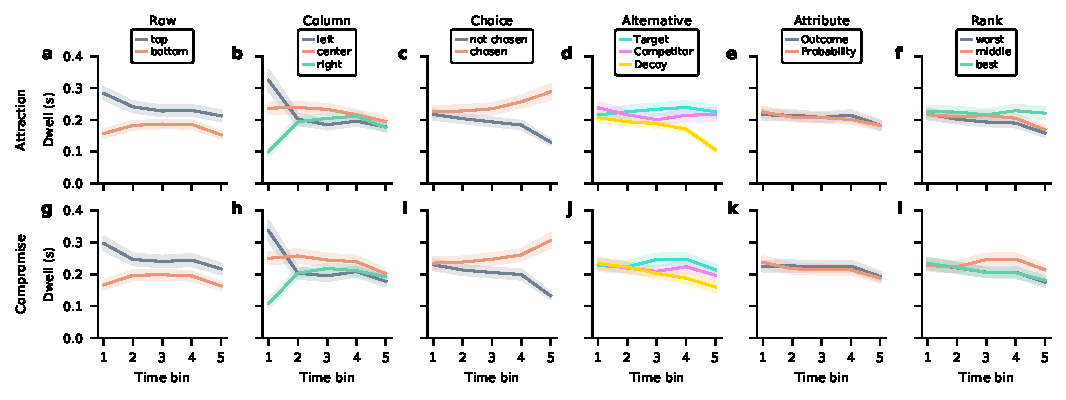
\includegraphics[scale=1]{../figures/S_gaze-data_timebinned_dwell.pdf}
\caption{\textbf{Distribution of gaze over the course of the trial depending on stimulus characteristics.} Each panel shows the average dwell time towards AOIs for a given stimulus feature (e.g., horizontal and vertical position) across five time-bins. Data is shown separately for attraction \textbf{(a-f)} and compromise \textbf{(g-l)} trials.}
\label{fig:dwell-data-timebinned}
\end{centering}
\end{figure}

\subsubsection*{Regression analyses of gaze behaviour}
We performed two linear mixed effects regressions of total dwell time towards an AOI in each trial, separate for attraction and compromise trials (Supplemental Figure \ref{fig:dwell-data-timebinned}). In the first ("full trial") model, the dependent variable was total dwell time towards an AOI across the full trial. This model used the following predictors: Vertical position (row, centred: -0.5 = top row, +0.5, bottom row), horizontal position (column, centred: -1 = left, 0 = centre, +1 = right), attribute (dummy coding probability attribute $p$), within dimension attribute rank (centred, -1 = worst, 0 = intermediate, +1 = best on attribute), target (dummy coded), decoy (dummy coded) and a dummy coded predictor for the ultimately chosen alternative. For the second model, we partitioned the dwell-data into five equally sized time-bins. The dependent variable in this model then was total dwell time towards an AOI within a time-bin. This model included the same predictors as the "full trial" model. Crucially, it also included interaction terms for each predictor with the time-bin variable, and time-bin as additional predictor. Both models included random intercepts and slopes for each participant. Bayesian posterior distributions of the regression weights were estimated using the bambi Python library \parencite{yarkoni2016BambiSimpleInterface}, with default priors \parencite{westfall2017StatisticalDetailsDefault}, sampling four chains with 2000 samples each, after a tuning phase of 500 samples. Convergence was diagnosed visually and by means of the Gelman-Rubin statistic ($|1 - \hat{R}| \le 0.05$ for all chains).

Regression weight estimates are shown in Supplemental Figure \ref{fig:dwell-regression-weights}. Across the trial, we find strong effects of position on dwell time, so that dwell times towards the top and left were longer. Significant negative interaction effects of the row and column predictors with time showed that these effects diminish across the trial. We also find a gaze-cascade effect \parencite{mullett2016ImplicationsVisualAttention,shimojo2003GazeBiasBoth}, where dwell times to AOIs belonging to the ultimately chosen alternative are longer across the trial (and increasingly so throughout the trial, indicated by the positive interaction term with time). Dwell times to decoys decreased significantly during the trial, and across the full trial, dwell times to decoys were shorter than other alternatives. Similarly, dwell times towards probability attributes p shortened across the trial. Across the full trial, however, dwell times towards probability AOIs were not shorter than those to outcome AOIs. Finally, dwell times to target alternatives were longer across the trial in both compromise and attraction trials. In addition, this effect increased throughout the trial in compromise, but not in attraction trials. Note that these effects are independent of the effect of choice, as choice is a separate predictor in the model. We could not find an association between the attribute rank (being the worst, best, or intermediate item on an attribute) and dwell time.

% Supplementary Figure: Dwell-regression weights
\begin{SCfigure}[0.8][t]
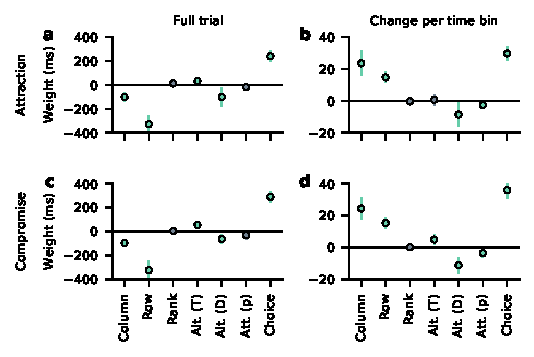
\includegraphics[scale=1]{../figures/S_dwell-regression_weights.pdf}
\caption{\textbf{Weight estimates from regression analyses on absolute dwell times.} We performed two mixed-effects regression analyses of dwell time towards each AOI onto stimulus properties: \textbf{(a, c)} Regressing the total dwell time towards an AOI over a full trial onto AOI column, row, attribute rank (best, middle or worst value on the attribute), two dummy predictors coding alternative, attribute (probability or outcome) and whether the AOI belonged to the subsequently chosen alternative. \textbf{(b, d)} Second, we binned dwell times in each trial into five time-bins and added an interaction term with time-bin for each predictor. The panels show the interaction term weights. Analyses were carried out separately for attraction \textbf{(a, b)} and compromise \textbf{(c, d)} trials. Regression models had random intercepts and slopes across participants. Points and intervals mark posterior mean estimates and associated HDI$_{95}$ (coloured green if the interval excluded 0).}
\label{fig:dwell-regression-weights}
\end{SCfigure}

\subsubsection*{Direction of information search}
We further analysed participants’ direction of information search. Therefore, we counted the number of vertical (transitions within the same alternative), horizontal (within the same row, between alternatives) and diagonal (between rows and alternatives) transitions. On average, participants made over 7 horizontal transitions in attraction (mean $\pm$ s.d. = 7.28 $\pm$ 2.36) and compromise (mean $\pm$ s.d. = 7.29 $\pm$ 2.63) trials, with no meaningful difference between effects. Participants made, however, more vertical transitions in compromise trials (mean $\pm$ s.d. = 7.55 $\pm$ 3.11) than attraction trials (mean $\pm$ s.d. = 7.17 $\pm$ 3.06; mean difference = 0.39, HDI$_{95}$  = [0.11, 0.64], $d$ = 0.49, HDI$_{95}$  = [0.13, 0.82]). The number of diagonal transitions was lower overall, but higher in attraction (mean $\pm$ s.d. = 2.88 $\pm$ 1.18) than compromise trials (mean $\pm$ s.d. = 2.72 $\pm$ 1.31; mean difference = 0.19, HDI$_{95}$  = [0.06, 0.32], $d$ = 0.62, HDI$_{95}$  = [0.14, 1.17]).

While vertical transitions always translate to transitions "within alternative", horizontal transitions are not necessarily always "within attribute", since the attribute positions of each alternative were random in the task. We therefore recoded transitions as "within alternative", "within attribute" and "between alternatives and attributes" and computed the Payne Index \parencite{payne1976TaskComplexityContingent} for each trial as:

\begin{equation}
    \text{Payne Index} = \frac{N_{\text{within~alt.}} - N_{\text{within~att.}}}{N_{\text{within~alt.}} + N_{\text{within~att.}}}
\end{equation}

A more positive value on the index indicates more processing within alternatives, whereas more negative values indicate more processing between alternatives, within the same attribute dimension. Overall, the average Payne Index was slightly positive for both attraction (mean $\pm$ s.d. = 0.10 $\pm$ 0.16) and compromise trials (mean $\pm$ s.d. = 0.14 $\pm$ 0.18), suggesting a mixture of within-alternative and within-attribute processing, with slightly more processing within alternatives. It was, however, lower in attraction trials (mean difference = 0.04, HDI$_{95}$  = [0.01, 0.06], $d$ = 0.51, HDI$_{95}$  = [0.17, 0.88]), implying comparably more processing between alternatives in attraction trials.
\clearpage

% Supplementary table: Summary of GLA estimates
\subsection*{GLA parameter estimates}
\begin{table}[h!]
\begin{centering}
\begin{tabular}{@{}llllllll@{}}
\toprule
       & mean & SD   & min  & 25\% & 50\% & 75\% & max   \\ \midrule
$\alpha$  & 0.47 & 0.35 & 0.05 & 0.25 & 0.37 & 0.61 & 1.67  \\
$\beta$   & 6.81 & 9.87 & 0.04 & 1.13 & 3.25 & 8.04 & 49.74 \\
$\gamma$  & 0.81 & 0.25 & 0.22 & 0.58 & 1.0  & 1.0  & 1.0   \\
$\lambda$ & 0.29 & 0.2  & 0.08 & 0.14 & 0.23 & 0.46 & 0.65  \\
$\theta$  & 0.69 & 0.18 & 0.13 & 0.63 & 0.72 & 0.83 & 0.95  \\ \bottomrule
\end{tabular}
\caption{\textbf{Summary of GLA estimates.} $\alpha$ is the utility parameter. $\beta$ is the inverse temperature parameter of the choice rule (0 = random choice). $\gamma$ is the probability weighting parameter (1 = objective probability weighting). $\lambda$ is the leak parameter (0 = perfect memory, 1 = full leak of all previous information). $\theta$ is the gaze-discount parameter (1 = no gaze-discount, 0 = maximum gaze-discount).}
\label{tab:gla-estimates}
\end{centering}
\end{table}
\clearpage

% Supplementary Figure: GLA estimates and correlations
\begin{figure}[ht!]
\begin{centering}
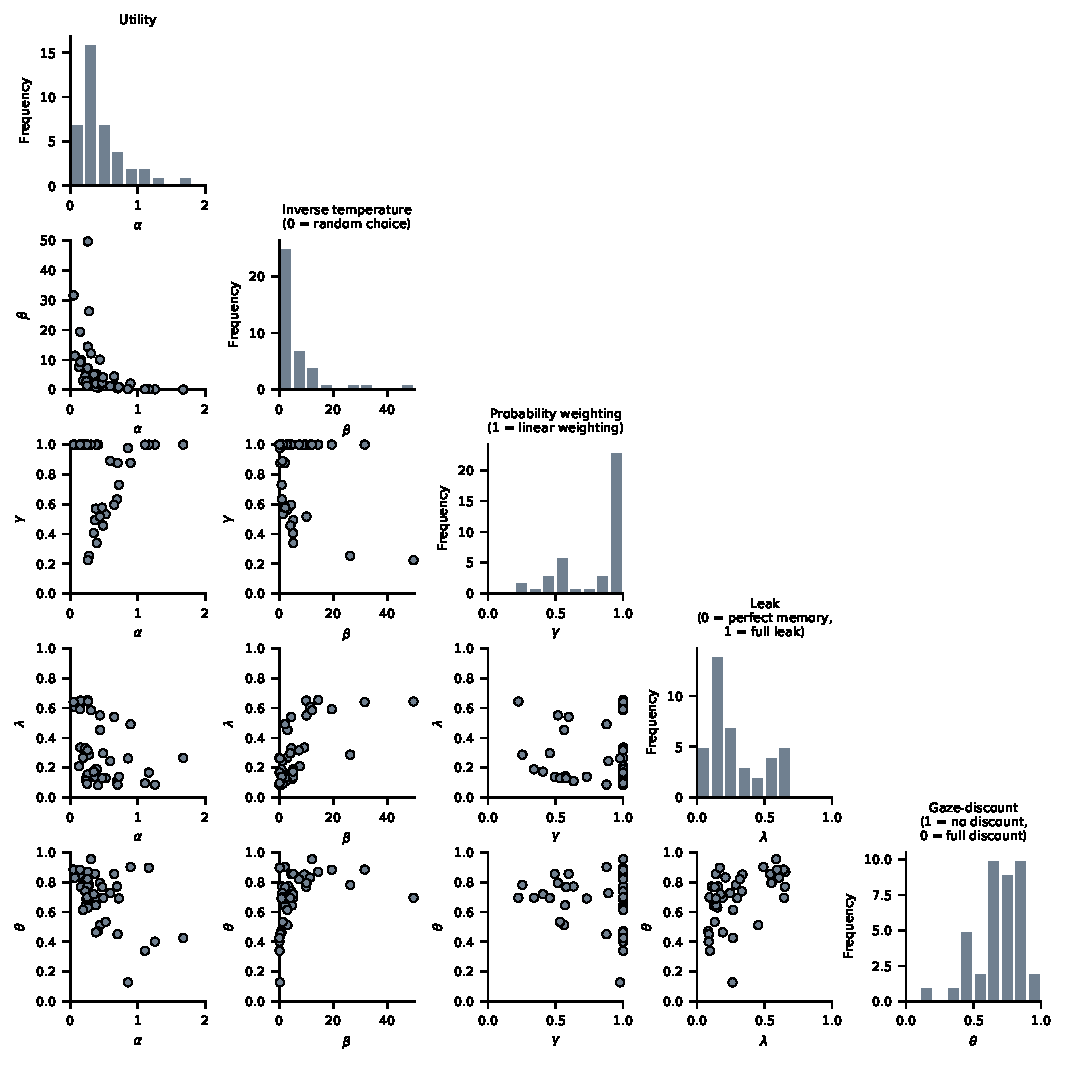
\includegraphics[scale=1]{../figures/S_gla-estimates.pdf}
\caption{\textbf{GLA maximum likelihood estimates and relationships between parameters.} $\alpha$ is the utility parameter. $\beta$ is the inverse temperature parameter of the choice rule (0 = random choice). $\gamma$ is the probability weighting parameter (1 = linear weighting). $\lambda$ is the leak parameter (0 = perfect memory, 1 = full leak of all previous information). $\theta$ is the gaze-discount parameter (1 = no gaze-discount, 0 = maximum gaze-discount).}
\label{fig:gla-estimates}
\end{centering}
\end{figure}
\clearpage

% Supplementary Figure: Model-predicted choice probabilities
\begin{figure}[ht!]
\begin{centering}
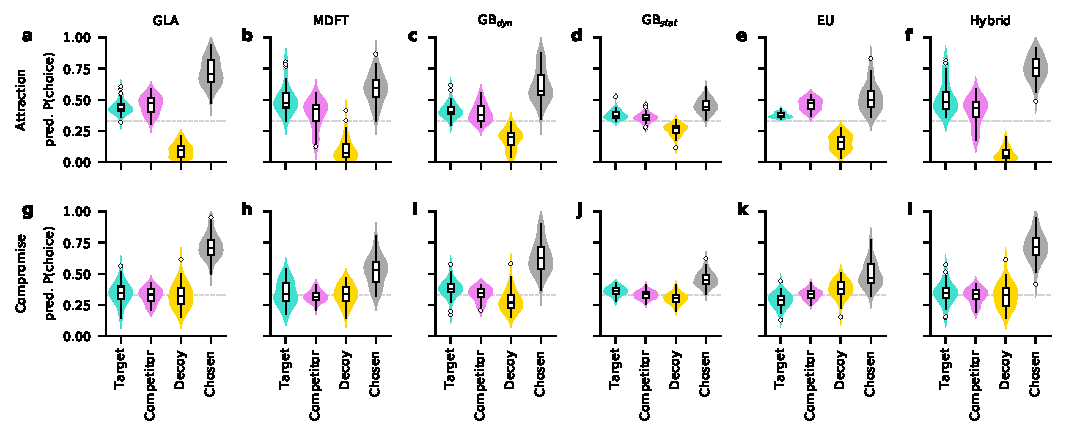
\includegraphics[scale=1]{../figures/S_model-predicted-choiceprobs.pdf}
\caption{\textbf{Model-predicted choice probabilities.} Each panel shows distributions of participant-level mean model-predicted choice probabilities for the target, competitor, decoy and ultimately chosen alternative. Predictions for attraction and compromise trials are displayed separately in the top \textbf{(a-f)} and bottom rows \textbf{(g-l)}. Predictions were computed using individual maximum likelihood estimates. The hybrid model \textbf{(f, l)} was derived from the switchboard analysis and combines an alternative-wise gaze-discount with a distance-dependent inhibition mechanism. Violin plots show kernel density estimates of distributions of individual values. Box plots mark lower and upper quartiles and median. Whiskers extend from first and last datum within 1.5 times the interquartile range from lower and upper quartiles, respectively. Values outside this range are indicated by open circles.}
\label{fig:model-pred-probs}
\end{centering}
\end{figure}
\clearpage

\subsection*{Context-effect strength and individual relative model fit}

% Supplementary Figure: Relative model fit and RST
\begin{figure}[ht!]
\begin{centering}
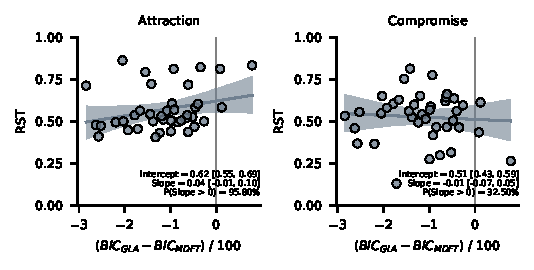
\includegraphics[scale=1]{../figures/S_GLA-vs-MDFT_dBIC_RST.pdf}
\caption{\textbf{Relative model fits between GLA and MDFT in relation to RST}. Relative model fits of MDFT (indicated by BIC difference between GLA and MDFT) tended to be higher for participants with higher RST in attraction trials (left panel; slope = 0.04, HDI$_{95}$ = [-0.01, 0.09] increase in RST per 100 unit increase in BIC difference, 93.6\% of posterior mass above 0), but not compromise trials (right panel), even though 7 out of 9 participants with attraction RST above 0.7 were better described by GLA overall (participants left of dashed vertical line).}
\label{fig:dbic-rst}
\end{centering}
\end{figure}
\newpage

% Supplementary Table: Switchboard Overview
\begin{sidewaystable}[ht]
\subsection*{Switchboard analysis overview}
\tiny
\begin{tabular}{@{}llllllllc@{}}
\toprule
\textbf{Switch} &
  \multicolumn{6}{c}{\textbf{Gaze-\emph{in}dependent levels}} &
  \multicolumn{1}{c}{\cellcolor[HTML]{DAE8FC}\textbf{Gaze-dependent levels}} &
  \textbf{N} \\ \midrule
\textbf{Attribute integration} &
  \multicolumn{3}{l}{\begin{tabular}[c]{@{}l@{}}$\times$ \textbf{Multiplicative}\\ Outcomes and probabilities\\ combine multiplicatively\\ into expected utilities.\\ \parencite{tversky1992AdvancesProspectTheory,glickman2019FormationPreferenceRisky}\end{tabular}} &
  \multicolumn{3}{l}{\begin{tabular}[c]{@{}l@{}}+ \textbf{Weighted additive}\\ Outcomes and probabilities\\ are normalized, weighted\\ and added.\\ \parencite{rouault2019PrefrontalMechanismsCombining}\end{tabular}} &
  \textit{n.a.} &
  2 \\ \midrule
\textbf{Comparison} &
  \multicolumn{3}{l}{\begin{tabular}[c]{@{}l@{}}\textbf{Independent}\\ Accumulation of absolute\\ item values per alternative.\\ \parencite{glickman2019FormationPreferenceRisky,bhatia2013AssociationsAccumulationPreference}\end{tabular}} &
  \multicolumn{3}{l}{\begin{tabular}[c]{@{}l@{}}\textbf{Comparative}\\ Accumulation of relative\\ values per alternative.\\ \parencite{roe2001MultialternativeDecisionField}\end{tabular}} &
  \textit{n.a.} &
  2 \\ \midrule
\textbf{Alternative-wise gaze-discount} &
  \multicolumn{6}{l}{\begin{tabular}[c]{@{}l@{}}\textbf{False}\\ Fixated and non-fixated alternatives processed equally.\end{tabular}} &
  \cellcolor[HTML]{DAE8FC}\begin{tabular}[c]{@{}l@{}}\textbf{True}\\ Non-fixated alternatives' values are\\ discounted by a parameter $\theta$.\\ \parencite[e.g.,][]{krajbich2010VisualFixationsComputation}\end{tabular} &
  2 \\ \midrule
\textbf{Attribute-wise gaze-discount} &
  \multicolumn{6}{l}{\begin{tabular}[c]{@{}l@{}}\textbf{False}\\ Fixated and non-fixated attributes are processed equally.\end{tabular}} &
  \cellcolor[HTML]{DAE8FC}\begin{tabular}[c]{@{}l@{}}\textbf{True}\\ Attributes on the non-fixated dimension\\ are discounted by a parameter $\eta$.\\ \parencite{krajbich2012AttentionalDriftdiffusionModel,fisher2017AttentionalDriftDiffusion}\end{tabular} &
  2 \\ \midrule
\textbf{Accumulation leak} &
  \multicolumn{3}{l}{\begin{tabular}[c]{@{}l@{}}\textbf{None}\\ Perfect integration over fixations.\end{tabular}} &
  \multicolumn{3}{l}{\begin{tabular}[c]{@{}l@{}}\textbf{Constant}\\ With each fixation, accumulators leak\\ information proportional to their current value,\\ controlled by parameter $\lambda$.\\ \parencite{roe2001MultialternativeDecisionField,usher2001TimeCoursePerceptual}\end{tabular}} &
  \cellcolor[HTML]{DAE8FC}\begin{tabular}[c]{@{}l@{}}\textbf{Gaze-dependent}\\ With each fixation, accumulators of\\ non-fixated alternatives leak information,\\ as in Constant leak.\\ \parencite{ashby2016FindingRightFit}\end{tabular} &
  3 \\ \midrule
\textbf{Accumulator inhibition} &
  \multicolumn{2}{l}{\begin{tabular}[c]{@{}l@{}}\textbf{None}\\ No inhibition between accumulators.\end{tabular}} &
  \multicolumn{2}{l}{\begin{tabular}[c]{@{}l@{}}\textbf{Constant}\\ Accumulators inhibit each other\\ proportional to their current value,\\ controlled by parameter $\Phi$.\\ \parencite{usher2004LossAversionInhibition}\end{tabular}} &
  \multicolumn{2}{l}{\begin{tabular}[c]{@{}l@{}}\textbf{Distance-dependent}\\ Inhibition between accumulators\\ depends on pairwise distance\\ between alternatives in attribute\\ space. Parameters $w_d$ and $\Phi$.\\ \parencite{roe2001MultialternativeDecisionField}\end{tabular}} &
  \cellcolor[HTML]{DAE8FC}\begin{tabular}[c]{@{}l@{}}\textbf{Gaze-dependent}\\ With each fixation, accumulators of\\ non-fixated alternatives are inhibited, \\ proportional to the currently fixated\\ accumulator's value.\\ Controlled by parameter $\Phi$.\end{tabular} &
  4 \\ \midrule
\textbf{Total variants} &
  \multicolumn{7}{l}{} &
  192 \\ \bottomrule
\end{tabular}
\caption{\textbf{Overview of the nodes and switch-levels used in the switchboard analysis.} Switch-levels that depend on gaze-data are shaded blue. Note that due to the model fitting procedure, where model predicted choice probabilities are derived from a soft-max function over the final accumulator values, the comparison switch levels \emph{independent} and \emph{comparative} are not distinguishable for a subset of the model space, reducing the total number of unique variants to 160.}
\label{tab:switchboard-overview}
\end{sidewaystable}
\clearpage

\subsection*{Best average fitting switchboard variants}
% Supplementary Table: Best average fitting (mean BIC) switchboard variants
\begin{table}[!ht]
\begin{centering}
\begin{tabular}{@{}cccccccc@{}}
\toprule
\textbf{Rank} & $\mathbf{GD_{Alt}}$                 & $\mathbf{GD_{Att}}$                 & \textbf{Leak}                         & \textbf{Inhibition}                   & \textbf{Integration}    & \textbf{Comparison}    & \textbf{BIC}    \\ \midrule
1    & \cellcolor[HTML]{DAE8FC}\textbf{Yes} & No                          & Constant                     & None                         & Multiplicative & \textit{n.d.} & 232.08 \\
2    & No                          & No                          & Constant                     & \cellcolor[HTML]{DAE8FC}\textbf{Gaze} & Multiplicative & Independent   & 235.94 \\
3    & \cellcolor[HTML]{DAE8FC}\textbf{Yes} & No                          & Constant                     & \cellcolor[HTML]{DAE8FC}\textbf{Gaze}                         & Multiplicative & Comparative   & 236.75 \\
4    & \cellcolor[HTML]{DAE8FC}\textbf{Yes} & \cellcolor[HTML]{DAE8FC}\textbf{Yes} & Constant                     & None                         & Multiplicative & \textit{n.d.} & 237.21 \\
5    & \cellcolor[HTML]{DAE8FC}\textbf{Yes} & No                          & Constant                     & \cellcolor[HTML]{DAE8FC}\textbf{Gaze} & Multiplicative & Independent   & 237.31 \\
6    & \cellcolor[HTML]{DAE8FC}\textbf{Yes} & No                          & Constant                     & Constant                     & Multiplicative & \textit{n.d.} & 237.40 \\
7    & \cellcolor[HTML]{DAE8FC}\textbf{Yes} & No                          & \cellcolor[HTML]{DAE8FC}\textbf{Gaze} & None                         & Multiplicative & Comparative   & 238.41 \\
8    & No                          & \cellcolor[HTML]{DAE8FC}\textbf{Yes} & Constant                     & \cellcolor[HTML]{DAE8FC}\textbf{Gaze} & Multiplicative & Independent   & 241.04 \\
9    & \cellcolor[HTML]{DAE8FC}\textbf{Yes} & No                          & Constant                     & Distance                     & Multiplicative & Comparative   & 241.40 \\
10   & \cellcolor[HTML]{DAE8FC}\textbf{Yes} & \cellcolor[HTML]{DAE8FC}\textbf{Yes} & Constant                     & \cellcolor[HTML]{DAE8FC}\textbf{Gaze} & Multiplicative & Comparative   & 241.78 \\ \bottomrule
\end{tabular}
\caption{\textbf{Overview of average best fitting model variants.} All ten model variants that fit the data best on average used some form of gaze-dependence (blue shaded cells), mostly an alternative-wise gaze discount. \textit{"n.d."} denotes variants where comparison mechanisms were not distinguishable by the analysis.}
\label{tab:switchboard-best-agg}
\end{centering}
\end{table}
\clearpage

\subsection*{Counts of individual best fitting switch levels}
% Supplementary Figure: Individual best fitting switch level counts
\begin{figure}[!ht]
\begin{centering}
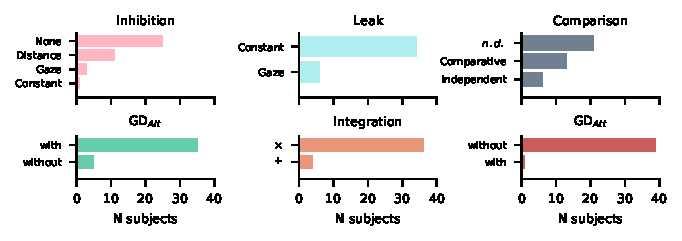
\includegraphics[scale=1]{../figures/S_switch-level_individual_counts.pdf}
\caption{\textbf{Counts of individual best fitting switches.} Most participants were best described by model variants that included multiplicative attribute integration, with alternative-wise gaze discount, no attribute-wise gaze discount, constant leakage and no inhibition.}
\label{fig:switchboard-ind-switch-counts}
\end{centering}
\end{figure}
\newpage


\subsection*{GLA and hybrid variant predicted choice probabilities by dwell time advantage for weak and strong attraction responders}
% Supplementary Figure: Relative dwell advantage for GLA and hybrid, subgroups (split by attraction effect strength)
\begin{figure}[!ht]
\begin{centering}
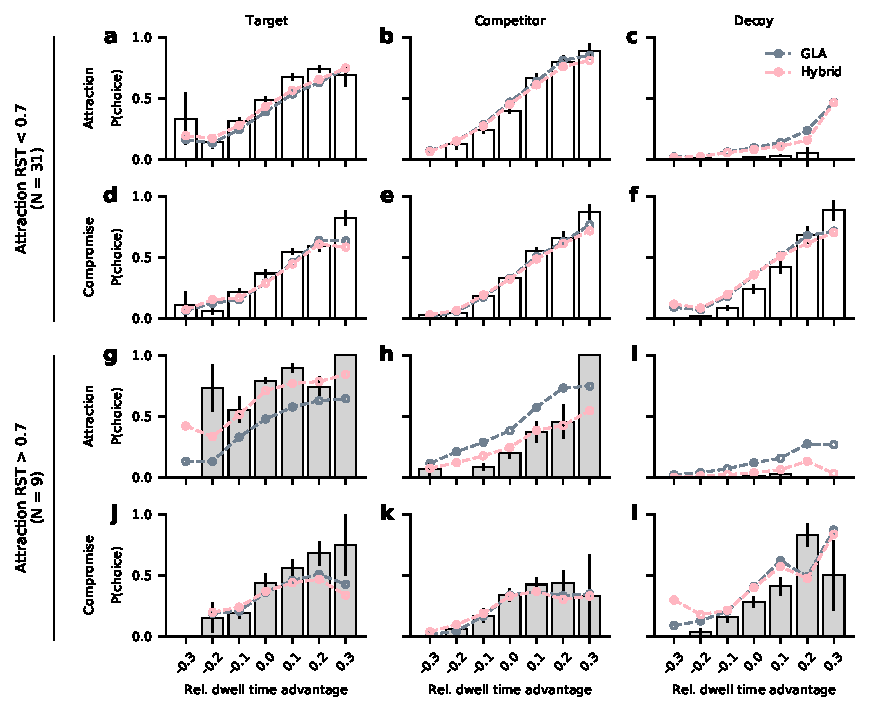
\includegraphics[scale=1]{../figures/S_dwell-advantage_subgroups_gla-hybrid.pdf}
\caption{\textbf{Observed and model-predicted association of dwell time advantage and choice for participants with weaker and strong attraction effects.} \textbf{(a-f)} Data and model predictions for participants with weaker attraction effects (RST $<$ 0.7). \textbf{(g-l)} Data and model predictions for participants with strong attraction effects (RST $>$ 0.7) Each column refers to one choice alternative: Target (first column; \textbf{a, d, g, j}); Competitor (second column; \textbf{b, e, h, k}); Decoy (third column; \textbf{c, f, i, l}). Rows refer to trials in attraction \textbf{(a-c, g-i)} and compromise trials \textbf{(d-f, j-l)}. White and grey bars and error bars show observed mean $\pm$ s.e. choice probabilities computed from even-numbered trials, for participants with weaker and stronger attraction effects, respectively. Coloured lines indicate model predictions derived from 50 simulations for each odd-numbered trial.}
\label{fig:rdt-adv-subgroups}
\end{centering}
\end{figure}
\newpage

\subsection*{No process evidence that strong attraction responders follow simple choice rule}
\label{sup:ade-choicerule}

Using process measures, we performed multiple tests of the hypothesis, that individuals with strong attraction effects follow a simple choice rule of choosing the dominant alternative. First, we tested whether the strength of individual attraction effects (individual RST in attraction trials) was related to differences in mean response times (RTs) in attraction trials. If individuals used a choice rule, their choices might be made faster, as they do not engage in multiple pairwise comparisons or calculations of expected outcomes. There was no correlation between the two measures ($r$ = 0.06, HDI$_{95}$ = [-0.24, 0.34]). Similarly, no relationship was found between individual RST and the number of fixations in attraction trials ($r$ = 0.07, HDI$_{95}$ = [-0.25, 0.37]). Mean RTs in attraction trials did not meaningfully differ between trials with target choices and trials with other choices ($d$ = -0.2, HDI$_{95}$ = [-0.67, 0.25]). Next, we tested whether individuals with strong attraction effects committed to a choice once they learned about the dominance relationship in the stimuli, as if using the dominance relationship as a stopping rule, or if they kept exploring the stimuli. There was, however, no relationship between individual RST and the mean number of fixations after all target and decoy attributes were fixated at least once ($r$ = 0.04, HDI$_{95}$ = [-0.27, 0.33]). The same analysis using fixation counts after target and decoy alternatives were both seen at least once on any attribute revealed no effect either ($r$ = 0.11, HDI$_{95}$ = [-0.20, 0.41]).
Taken together, we did not find any evidence based on process data to support the hypothesis that strong attraction responders used a simple choice rule.

\end{document}
